

\documentclass{article}
\usepackage[utf8]{inputenc}
% Better font encoding for French and scalable fonts
\usepackage[T1]{fontenc}
\usepackage{lmodern}
\usepackage{amsmath, amssymb, amsfonts, amsthm, stmaryrd}
\usepackage{tikz}
\usetikzlibrary{matrix,arrows}
\usepackage{tikz-cd}
\usepackage{geometry}
\usepackage[french]{babel}
\usepackage{amsopn}

\title{Étude de manoeuvres orbitales de satellites - draft}
\author{Etienne Chevrolat}
\date{}


\begin{document}

\maketitle

\begin{abstract}
    Dans cette étude, on cherche à caractériser les différents Patterns of Life (PoL) de satellites en orbites géosynchrone (GEO) et basse altitude (LEO).
    Pour cela, on se base sur de l'analyse de données TLE issues de SpaceTrack ainsi que sur le travail de chercheurs au MIT ArcLab, premiers concepteurs d'un dataset public GEO labellisé, SPLID.
    Cependant, il est bon de noter que le dataset SPLID contient des données majoritairement simulées. Nous allons donc ici nous inspirer de leur travail pour tenter de caractériser des PoL de données réelles issues de satellites en orbites GEO et LEO.
\end{abstract}

\section{Le type de données }

\subsection{Les paramètres orbitaux}

Les orbites des satellites sont elliptiques, caractérisées par leurs éléments keplériens :

\vspace{0.3cm}
\noindent\fbox{%
\begin{minipage}{0.98\textwidth}

\textbf{Paramètres orbitaux}
\begin{itemize}
    \item a : semi-grand axe de l'ellipse
    \item e : excentricité de l'ellipse
    \item i : inclinaison de l'ellipse
    \item $\omega$ : argument du périgée
    \item $\Omega$ : Right Ascension of Ascending Node
    \item M : anomalie moyenne, renseigne sur la position du satellite sur son orbite à un instant t 
\end{itemize}
\end{minipage}

}
\vspace{0.5cm}

On peut ensuite lier des variations de vitesse dans le référentiel inertiel terrestre aux variations des paramètres orbitaux de l'ellipse, et vice-versa. 

\vspace{0.3cm}

\noindent\fbox{
\begin{minipage}{0.98\textwidth}
\textbf{Variations de vitesse et variations de paramètres orbitaux}\newline
On considère une variation $\Delta v = (\Delta v _r , \Delta v _u ,\Delta v _h )$ de la vitesse décomposée dans le référentiel terrestre en vitesses radiale, tangentielle et normale.
Les équations de Gauss nous donnent dans la limite quasi-circulaire:  
\begin{itemize}
    \item $\Delta a = \dfrac{2}{n} \Delta v _u$
    \item $\Delta e = \dfrac{1}{na}(\sin f \Delta v _r  + 2 \cos f \Delta v_u )$
    \item $\Delta i = \dfrac{1}{na}(\cos (\omega + f)  \Delta v _h  )$
    \item $\Delta \Omega  = \dfrac{1}{na}(\dfrac{\sin (\omega + f )}{\sin i }\Delta v _h  )$
    \item $\Delta \omega =  \dfrac{1}{na e }( - \cos f \Delta v _r   + 2 \sin f \Delta v_u ) - \Delta \Omega \cos i $
\end{itemize}
\end{minipage}

}
\vspace{0.3cm}

On en déduit les interprétations suivantes : 
Des variations de a et e traduisent des manoeuvres \textit{in plane}  (variation de vitesse radiale)
Des variations de i et $\Omega$ traduisent des  manoeuvres \textit{out plane} (variation de vitesse normale)

\subsection{Two Line Elements}

Les paramètres orbitaux décrits ci-dessus ne sont pas mesurés directement : ils sont diffusés par les organismes de surveillance de l'espace sous la forme de \textit{Two Line Elements} (TLE).
Un TLE est un format standardisé qui encode, sur deux lignes de 69 caractères, l'ensemble des éléments nécessaires pour reconstituer l'orbite d'un objet à un instant de référence appelé \textit{epoch}.

\vspace{0.3cm}
\noindent\fbox{%
\begin{minipage}{0.98\textwidth}

\textbf{Contenu d'un TLE}
\begin{itemize}
    \item \textbf{Identification} : numéro de catalogue NORAD, classification, désignateur international (année de lancement, numéro de lancement) et numéro du jeu d'éléments.
    \item \textbf{Epoch} : date de référence à laquelle les éléments sont valides, exprimée en année et fraction de jour.
    \item \textbf{Éléments orbitaux} : inclinaison $i$, ascension droite du noeud ascendant $\Omega$, excentricité $e$, argument du périgée $\omega$, anomalie moyenne $M$ et moyen mouvement $n$ (en révolutions par jour).
    \item \textbf{Termes de perturbation} : dérivées première et seconde du moyen mouvement ($\dot n$, $\ddot n$) et coefficient de traînée atmosphérique $B^*$.
\end{itemize}
\end{minipage}

}
\vspace{0.5cm}

Il est important de noter que les éléments contenus dans un TLE ne sont pas des éléments osculateurs (l'orbite képlérienne instantanée), mais des \textit{éléments moyens} : les perturbations périodiques à courte période en ont été retirées.
Ils ne sont donc exploitables qu'avec le modèle de propagation qui a servi à les générer.

Ce modèle est le \textbf{SGP4} (\textit{Simplified General Perturbations 4}), un propagateur analytique qui prend en entrée un TLE et fournit la position et la vitesse du satellite dans le référentiel inertiel terrestre à n'importe quel instant.
Contrairement à une simple propagation képlérienne, SGP4 tient compte des principales perturbations subies par l'orbite : l'aplatissement terrestre (harmoniques zonaux $J_2$, $J_3$, $J_4$), la traînée atmosphérique via le terme $B^*$ ainsi que les effets à longue période.


\section{Caractérisation de PoL}
\par 
On se base sur l'API SpaceTrack pour récupérer les données souhaitées sous format TLE. Cet outil a été créé pour avoir un contrôle maximal sur les données récupérées.
Lors de la requête, on peut choisir le pays d'origine des satellites ainsi que la constellation à laquelle ils appartiennent, si elle est documentée publiquement (par exemple Starlink ou OneWeb).
On peut également choisir les dates de début et de fin d'acquisition si l'on veut constituer un historique de données orbitales.
Enfin, on peut choisir la range du demi-grand axe des orbites récupérées, ce qui permet d'obtenir uniquement des données de satellites en LEO, MEO ou géostationnaires.

\subsection{Données GEO}

\par       
Un type de donnée particulièrement important pour nous est celui des satellites géostationnaires.
Leur orbite est théoriquement fixée à 35 786 km au-dessus de la Terre, soit un rayon de l'orbite de 42 164 km.
Une fois placé sur cette orbite, le satellite est quasi-immobile dans le référentiel terrestre, ce qui lui permet de suivre une position fixe de latitude et longitude. 
La non-sphéricité de la Terre et le fait que les orbites ne soient pas purement circulaires (excentricité très faible mais non nulle) imposent cependant une dérive de certains paramètres orbitaux.


Pour maintenir les satellites GEO sur leur position souhaitée, les opérateurs peuvent par exemple effectuer des manoeuvres dites de station-keeping, 
\begin{itemize}
    \item Est-Ouest (manoeuvres in plane)
    \item Nord-Sud (manoeuvres out plane)
\end{itemize}

\par 
Des chercheurs du MIT ont défini le premier jeu de données de manoeuvres labellisé de satellites GEO (SPLID) conséquent,
dans le but de fournir un dataset utilisable pour entraîner des modèles à reconnaître les différentes manoeuvres.
Ils définissent donc les PoL des satellites par : 
\begin{itemize}
    \item Des noeuds (nodes) de PoL, i.e. des points de rupture au sein du PoL
    \item Des behavioral modes, i.e. valeurs catégorielles entre deux noeuds de PoL 
\end{itemize}
Des noeuds de type Initiate Drift (déclenchement d'une dérive) ID, Adjust Drift(correction de dérive) AD, et Initiate Station-Keeping (Début de maintien à poste) IK sont ainsi définis. 
Les noeuds Start of Study period SS et End of Study period ES sont également définis mais ne correspondent pas physiquement à des manoeuvres, simplement indique le début/fin de l'acquisition du PoL du satellite.


Parmi les behvaioral modes correspondant à des manoeuvres de station-keeping (SK), les chercheurs ont différencié le type d'impulsion (chimique CK, électrique EK, hybride HK). 
Tous ce qui n'est pas de station keeping est de type not station-keeping (NK). 
Les différentes PoLs sont résumés dans la Table 1 :

\begin{center}
    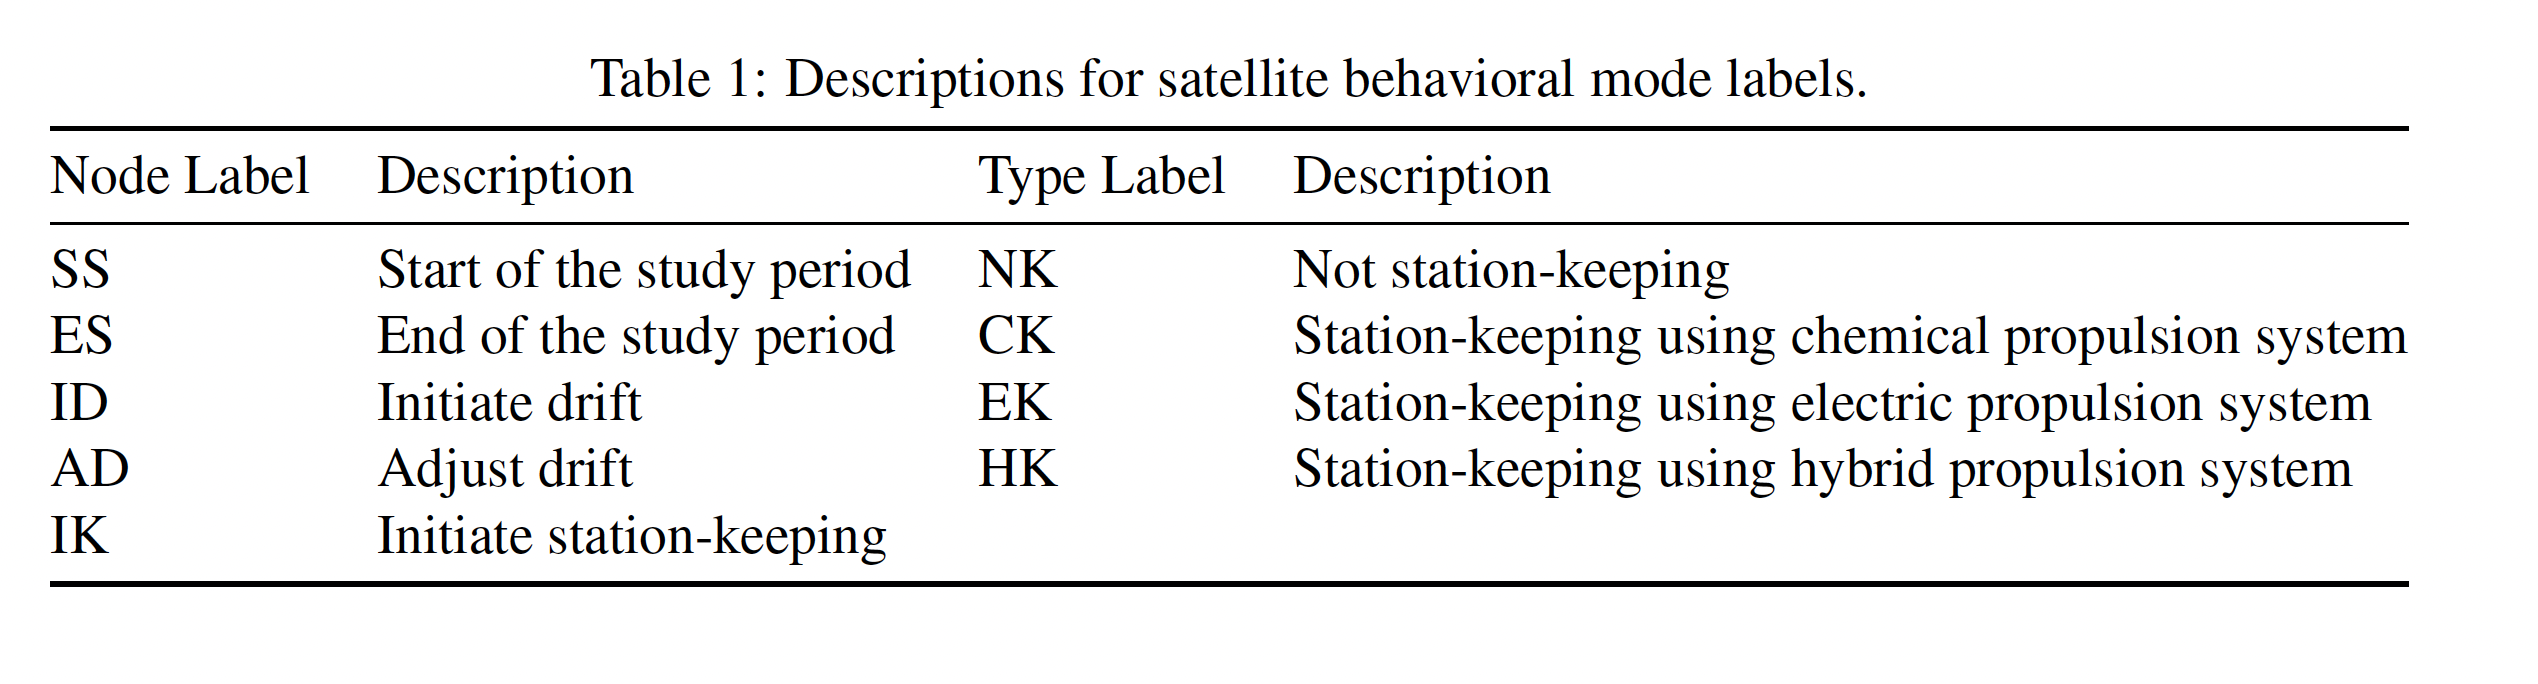
\includegraphics[scale=0.3]{figures/Capture d’écran 2026-07-01 à 14.41.14.png}
\end{center}

Ci-dessous sont tracés les paramètres orbitaux et différents noeuds correspondant aux PoL du satellite Horizons 2, NORAD 32388.
Les lignes verticales correspondent aux différents behavioral modes tandis que les marqueurs circulaires indiquent les noeuds de PoL directionnels dans leurs domaines respectifs.

\begin{center}
    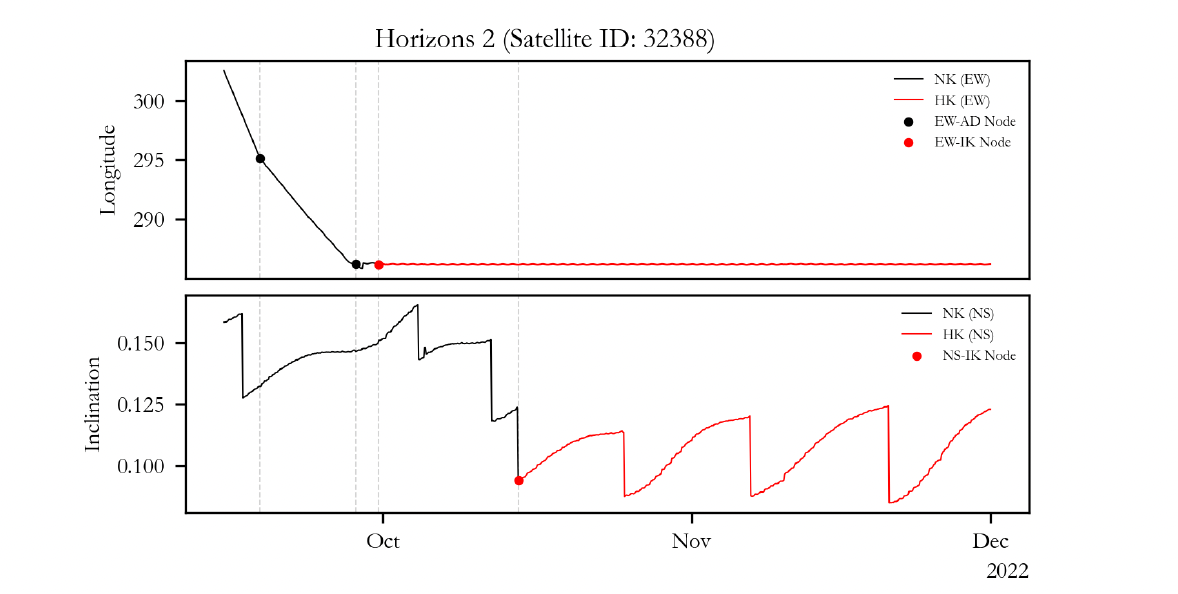
\includegraphics[scale=0.7]{figures/Capture d’écran 2026-07-01 à 14.41.03.png}
\end{center}

Voici un résumé des noeuds de PoL d'un satellite du dataset.

\begin{center}
    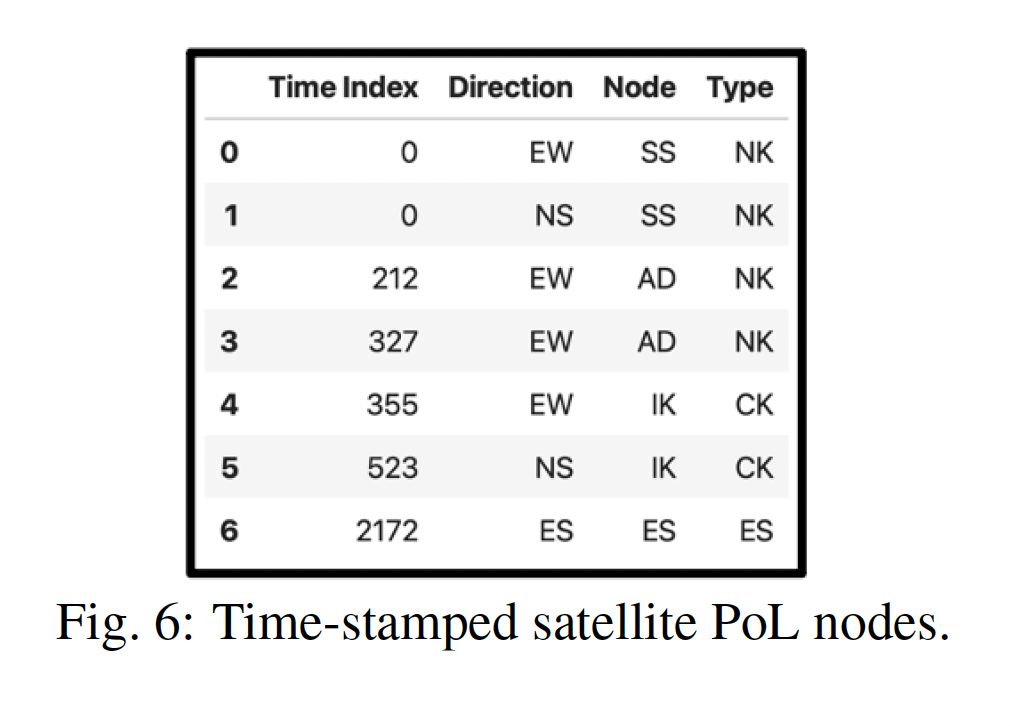
\includegraphics[scale=0.4]{figures/Capture d’écran 2026-07-01 à 14.41.33.png}
\end{center}

\subsubsection{Manoeuvres des des satellites GEO}

On essaye maintenant de se focaliser sur des manoeuvres de type station-keeping issues de données réelles. On a d'ores et déjà constitué un dataset exploitable de l'historique de TLE de $\sim$200 satellites GEO issus de tous les pays.
On examine deux satellites en guise d'exemple :
\begin{itemize}
    \item 43226 : Satellite US. "GOES-17 is a geostationary weather satellite designed to improve the forecasts of weather, ocean, and environment by providing faster and more detailed data, real-time images of lightning, and advanced monitoring of solar activities and space weather"
    \item 66142 : Satellite Chinois (aucune info)
\end{itemize}

On trace alors leur demi-grand axe $a$ et le résultat de notre V1 de 3 outils de détection de manoeuvres :
\begin{itemize}
    \item (MLF KEPLER) Une méthode GEO basée sur les résidus de la longitude moyenne $\lambda = \Omega + \omega + M$, avec une propagation keplerienne naive.
    \item (MLF SPG4) Une méthode GEO basée sur les résidus de la longitude moyenne, avec une propagation SGP4.
\end{itemize}

Sur le graphe du demi-grand axe, c'est le résultat de notre algo implémentant un filtre Kalman qui est représenté.

\begin{center}
    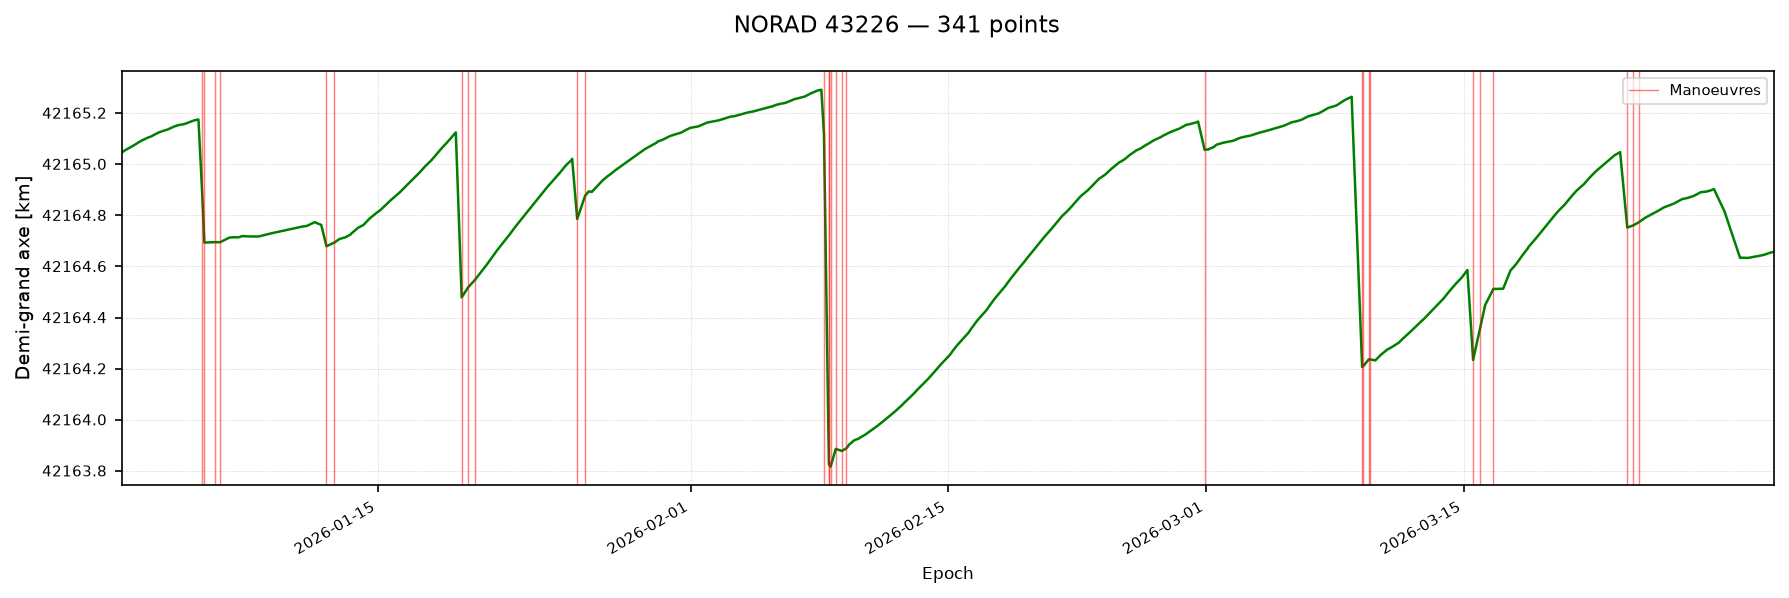
\includegraphics[scale=0.5]{figures/norad_43226_sma_and_maneuvers copy.png}
    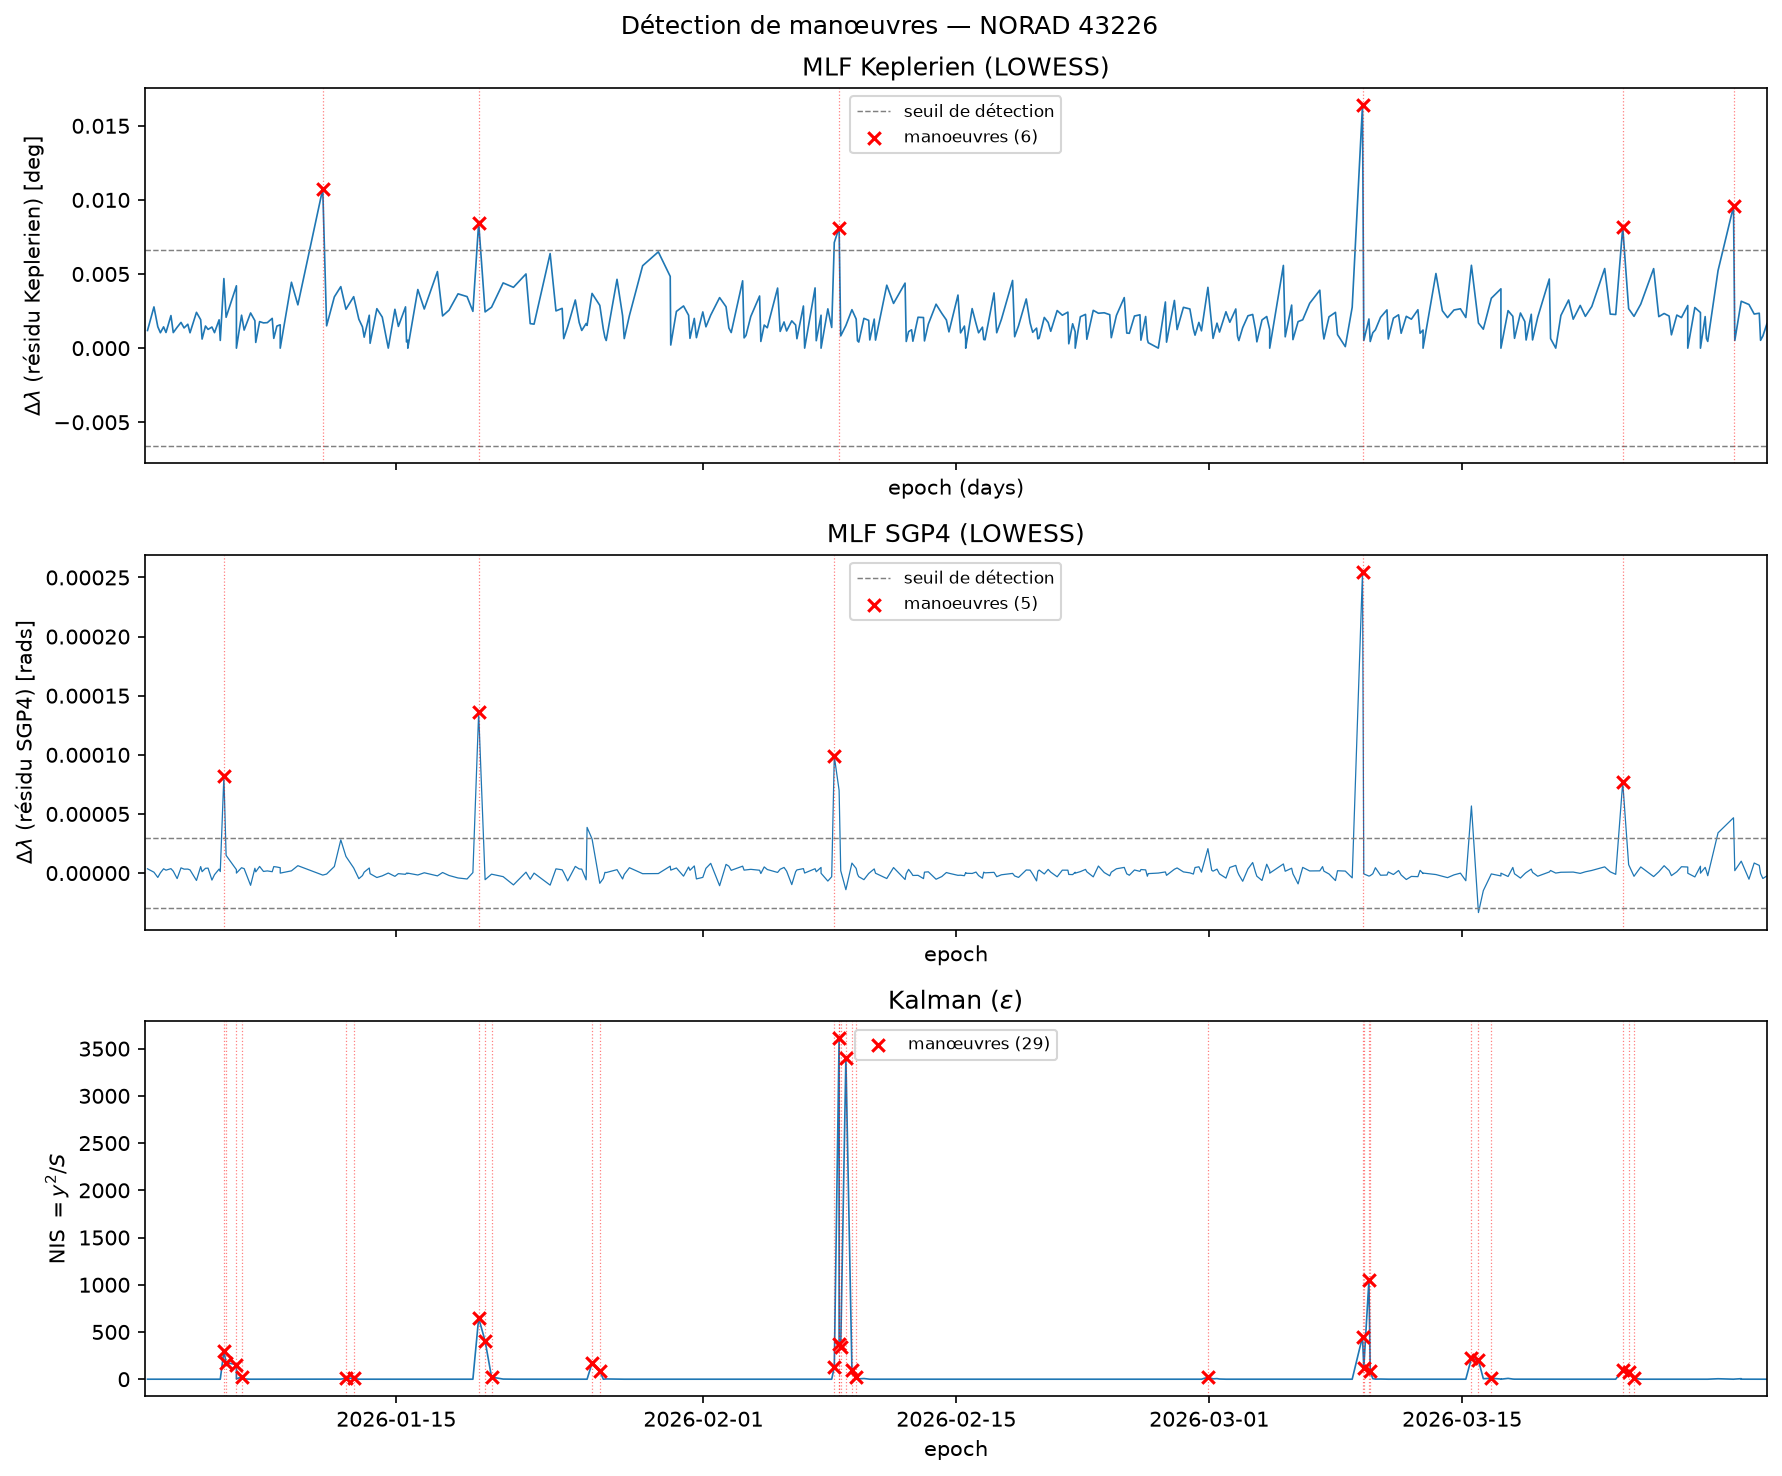
\includegraphics[scale=0.4]{figures/norad_43226_methods.png}
\end{center}

\begin{center}
    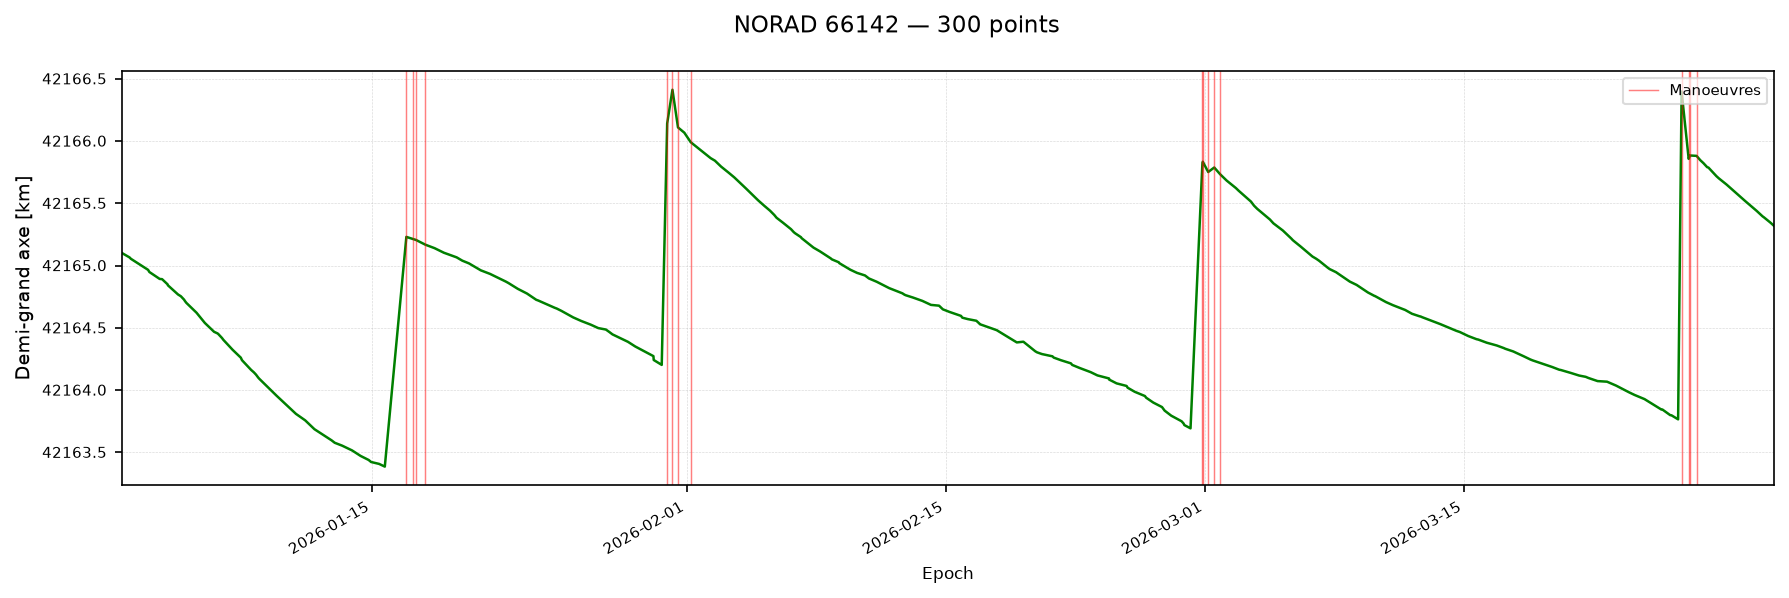
\includegraphics[scale=0.5]{figures/norad_66142_sma_and_maneuvers copy.png}
    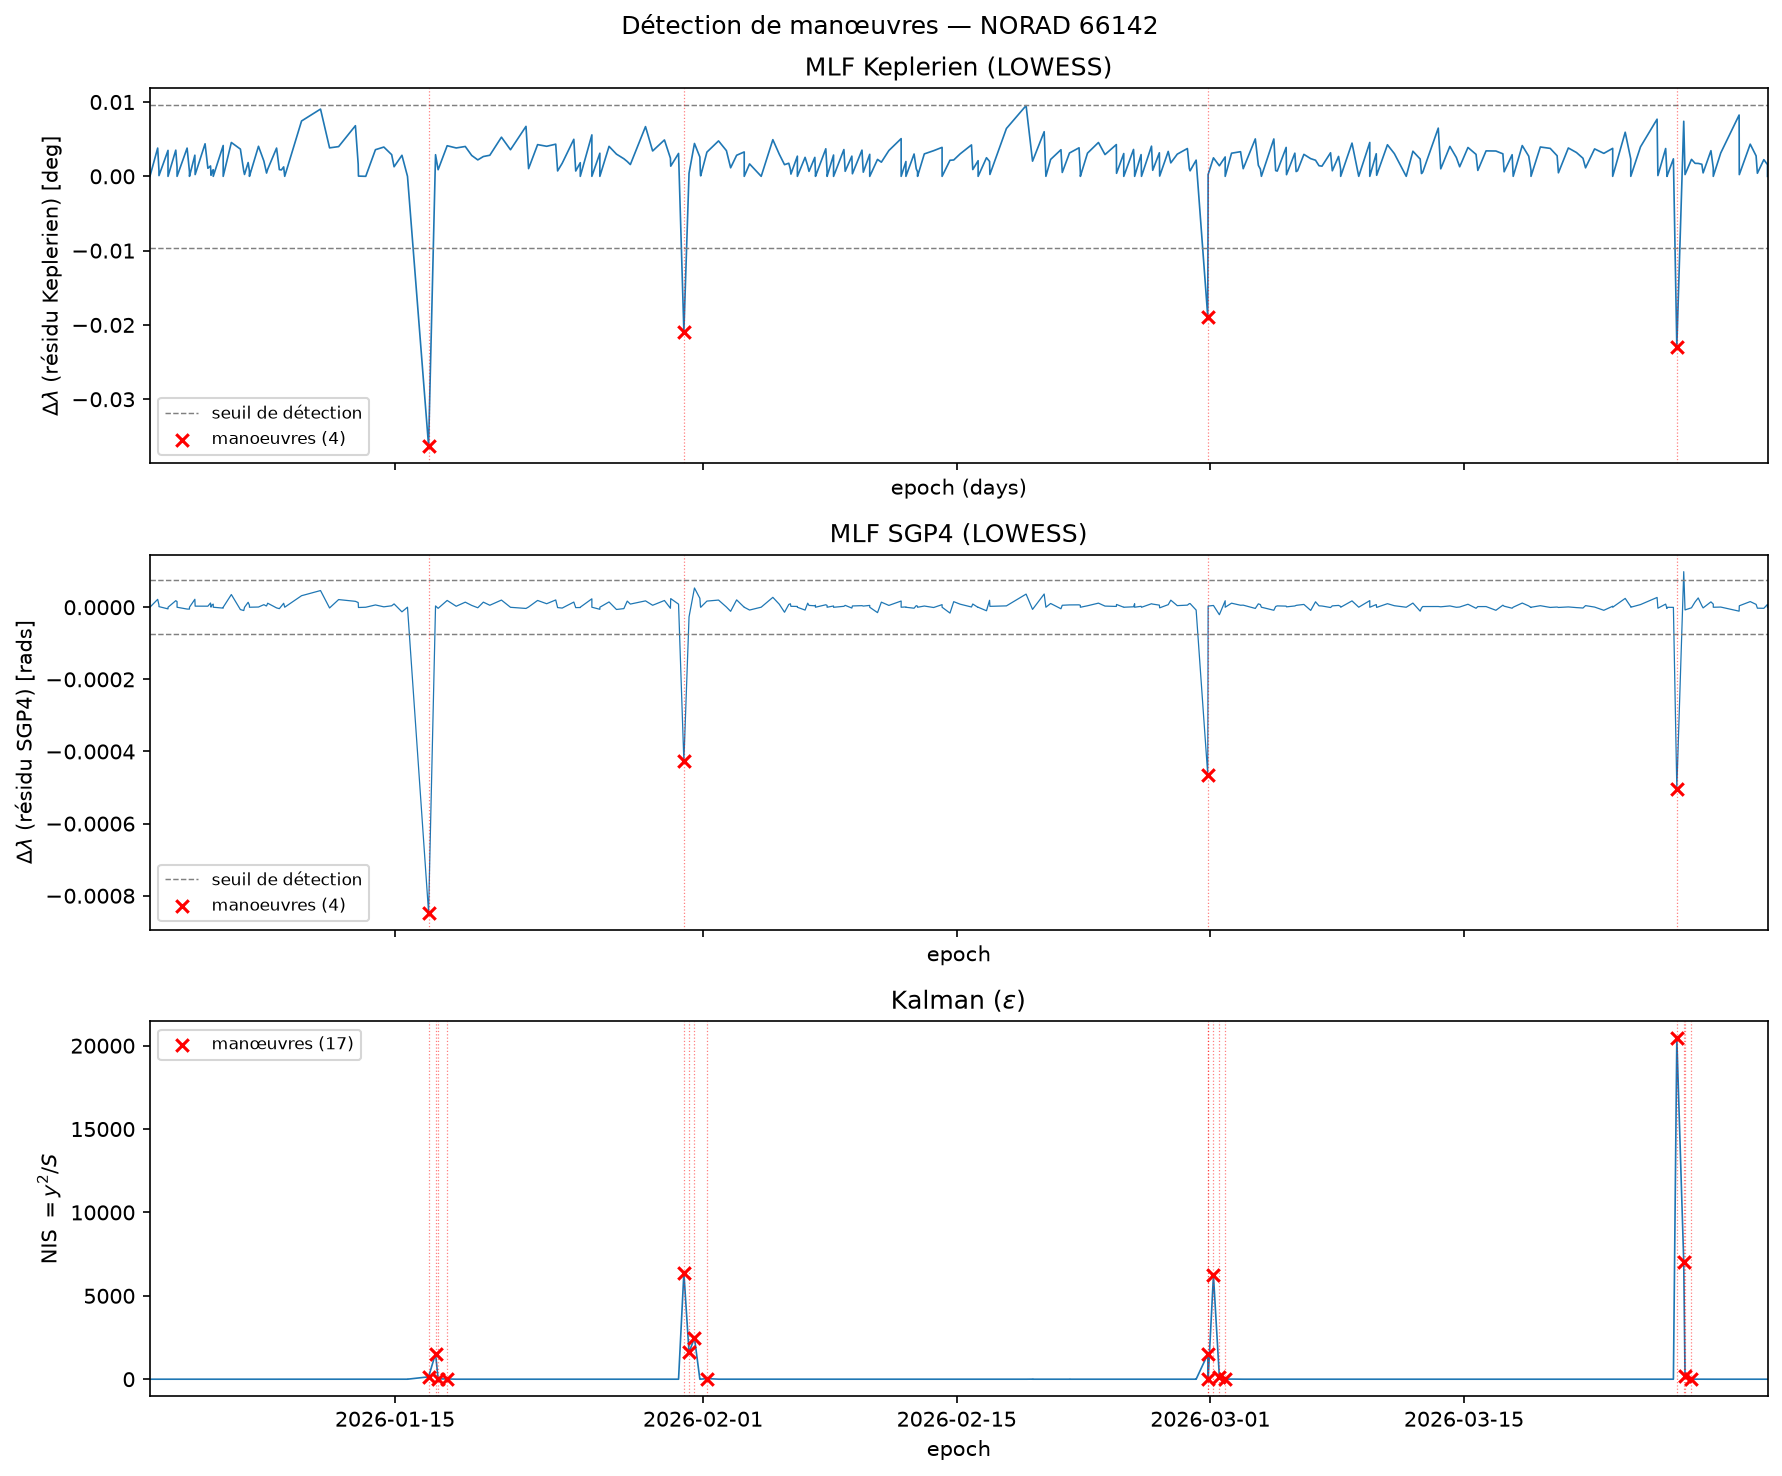
\includegraphics[scale=0.4]{figures/norad_66142_methods.png}
\end{center}

\textbf{Remarques:}
Pour l'instant, on ne différencie pas le type de manoeuvres détectées grâce à ces différentes méthodes.
Cependant, la méthode par filtrage de Kalman est basée sur le demi-grand axe : on est donc en train de mesurer des manoeuvres in-plane.
Les méthodes Mean Longitude Filter sont basées sur la longitude moyenne $\lambda = \Omega + \omega + M$ et détectent aussi des manoeuvres in plane. 

\subsubsection{A suivre :} 
\begin{itemize}
    \item en GEO, les algos de détection de manoeuvres doivent préciser clairement le type de manoeuvres opérées (NS, EW, Station-Keeping ou non). 
    \item poursuivre l'étude de PoL en LEO, plus complexes a priori, qui ne contiennent pas seulement des manoeuvres de station-keeping
    \item effectuer des mesures quantitatives de manoeuvres (intensité de la manoeuvre, via calcul de $\Delta v$ ?)
    \item implémenter d'autres méthodes classiques de détection de manoeuvres
    \item le problème du seuillage ressort constamment lorsque l'on utilise des méthodes classiques de détection de manoeuvres. Il y a toujours une part arbitraire lors de sa calibration qui nécessite souvent du cas par cas et empêche une bonne automatisation, d'où la volonté de s'intéresser à des méthodes de ML.
\end{itemize}


\subsection{Données LEO}

\subsubsection{Les données de manoeuvres ILRS}

L'ILRS (\textit{International Laser Ranging Service}) met à disposition, en libre accès, des historiques de manoeuvres réelles pour les satellites suivis par télémétrie laser.
Ces données constituent un jeu de données labellisé solide, issu de mesures réelles et non de simulations, contrairement à la majorité du dataset SPLID.

Chaque ligne d'un fichier de manoeuvres ILRS contient :
\begin{itemize}
    \item l'identifiant du satellite (par exemple CRYO2 pour CryoSat-2) ;
    \item les dates de début et de fin de la manoeuvre ;
    \item le type de paramètres fournis ;
    \item le nombre de burns, puis pour chaque burn : la date médiane, la durée du boost, les trois composantes de la variation de vitesse $(\Delta v_r, \Delta v_u, \Delta v_h)$, les trois composantes de l'accélération et les écarts d'accélération par rapport à la prédiction.
\end{itemize}

Les satellites dont les manoeuvres sont documentées (SPOT, TOPEX, Jason, Envisat, CryoSat-2, SARAL, Sentinel-3) sont tous en orbite basse : la base de données ILRS ne fournit donc que des données de satellites LEO.

\subsubsection{Confrontation aux séries temporelles TLE}

On superpose les dates de manoeuvres ILRS aux séries temporelles des paramètres orbitaux issus des TLE SpaceTrack, pour quatre satellites : Sentinel-3B (NORAD 43437), Envisat (NORAD 27386), CryoSat-2 (NORAD 36508) et SARAL (NORAD 39086).
Les acquisitions se sont faites sur des intervalles de temps variables selon les satellites. 
\subsubsection{Sentinel-3B (NORAD 43437)}

\begin{center}
    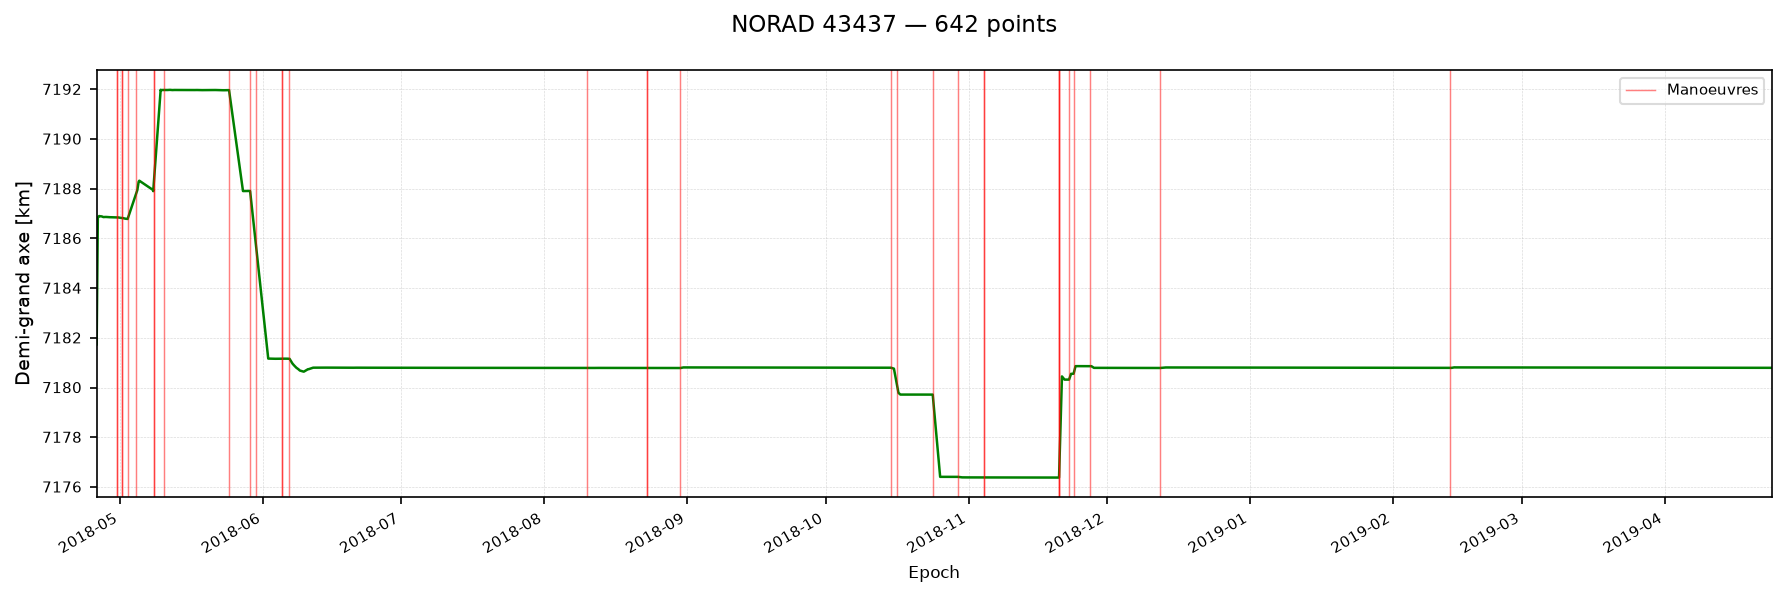
\includegraphics[width=0.48\textwidth]{figures/s3b_sma.png}
    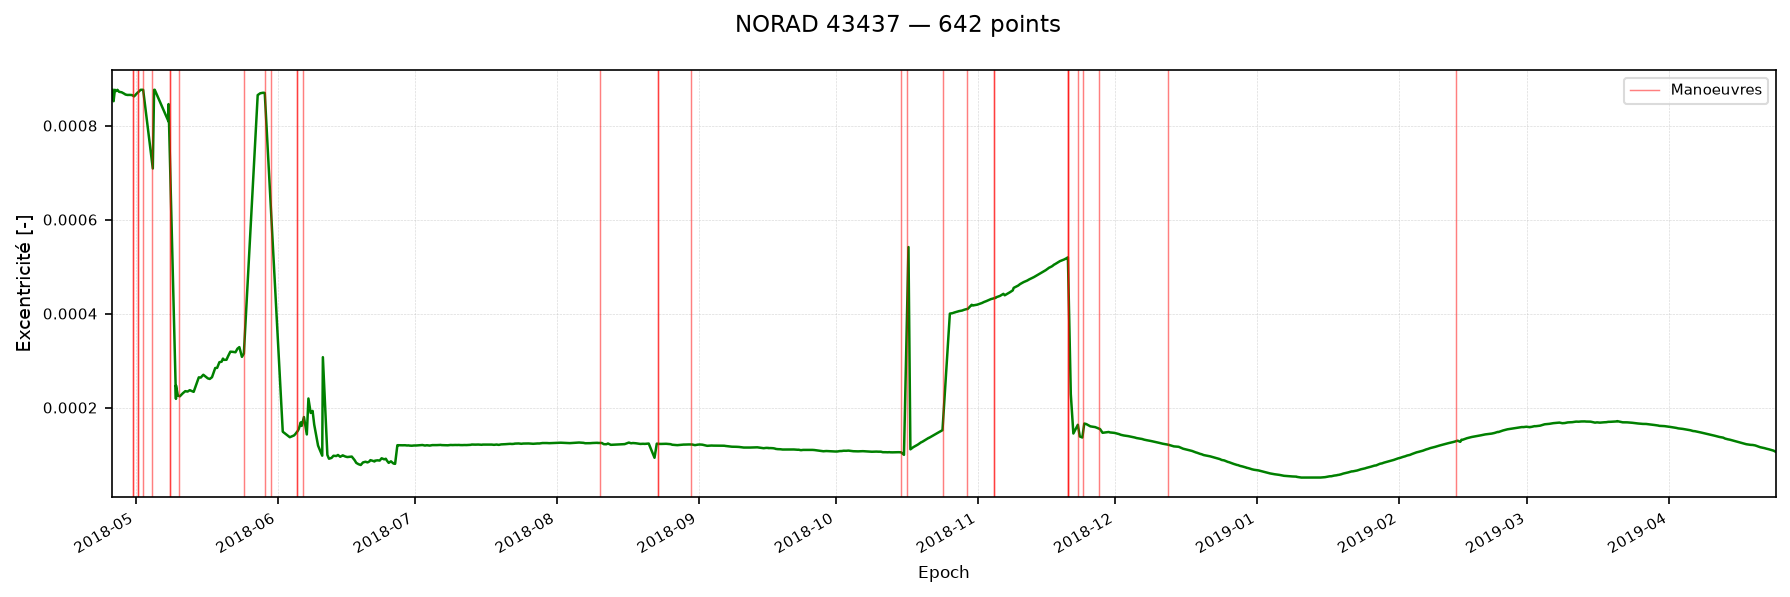
\includegraphics[width=0.48\textwidth]{figures/s3b_eccentricity.png}
    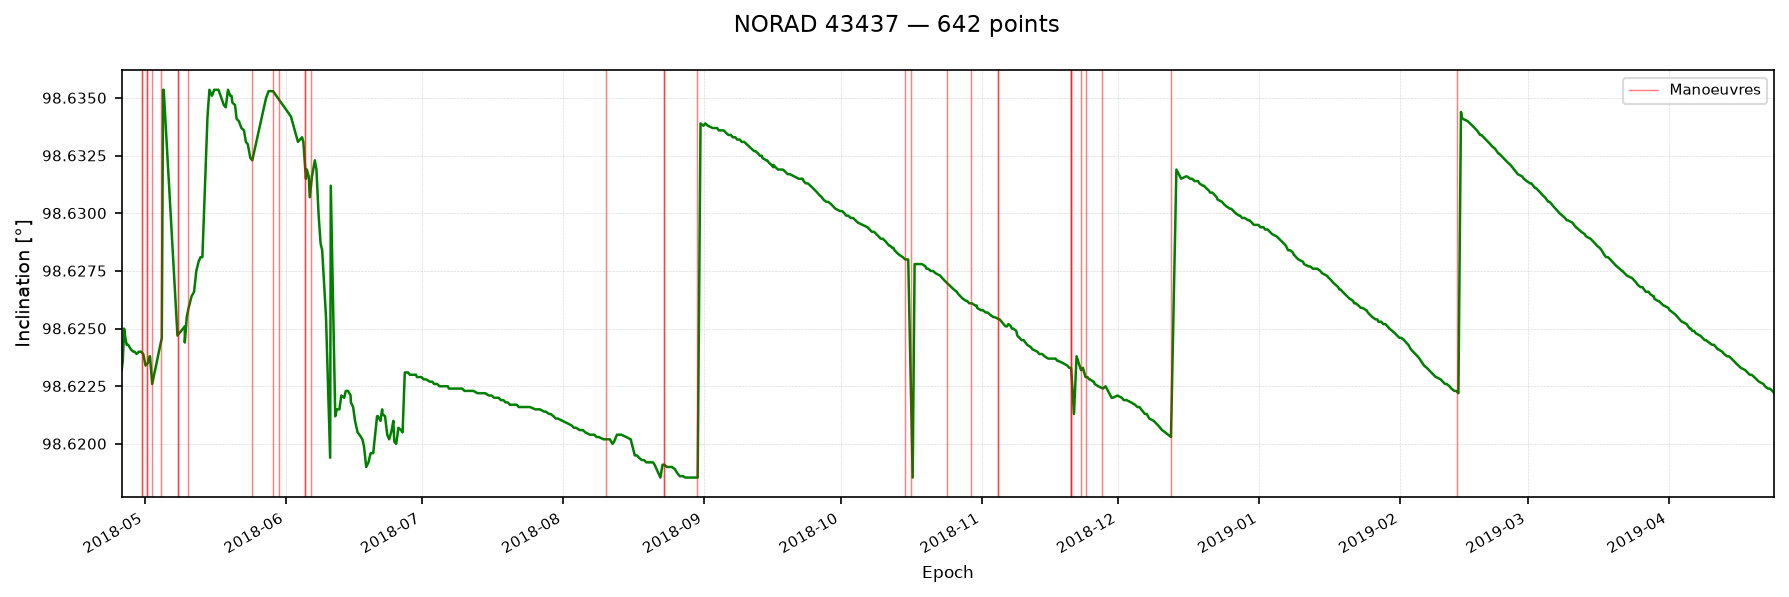
\includegraphics[width=0.48\textwidth]{figures/s3b_inclination.png}
    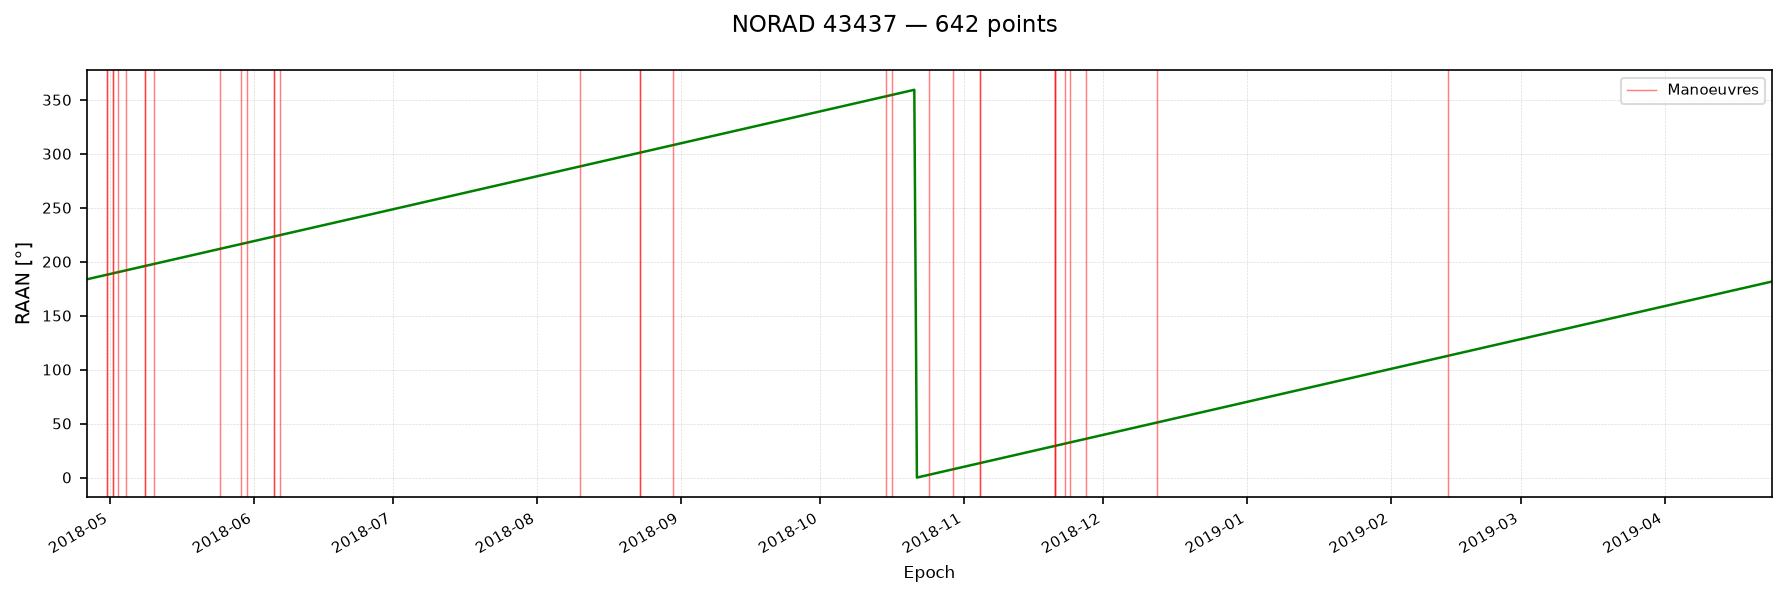
\includegraphics[width=0.48\textwidth]{figures/s3b_raan.png}
    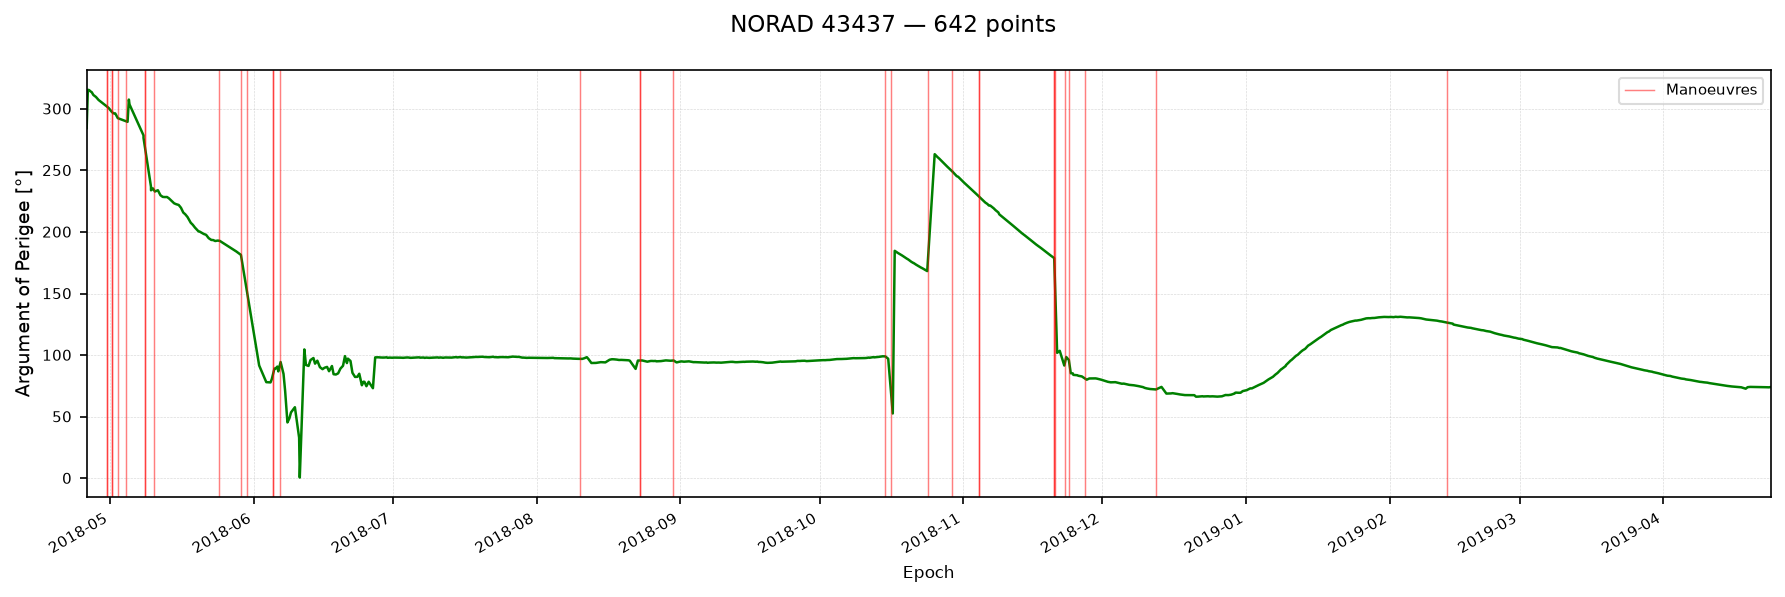
\includegraphics[width=0.48\textwidth]{figures/s3b_arg_perigee.png}
    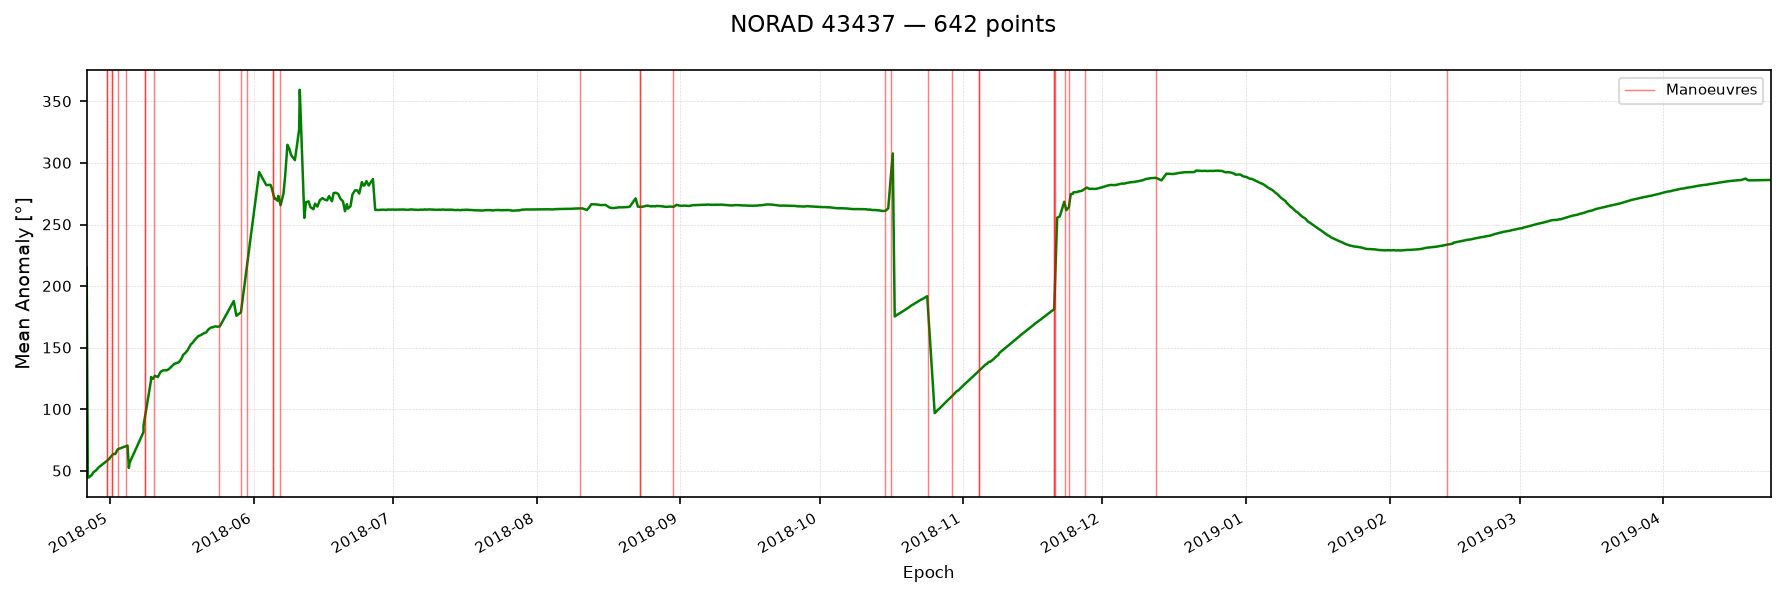
\includegraphics[width=0.48\textwidth]{figures/s3b_mean_anomaly.png}
    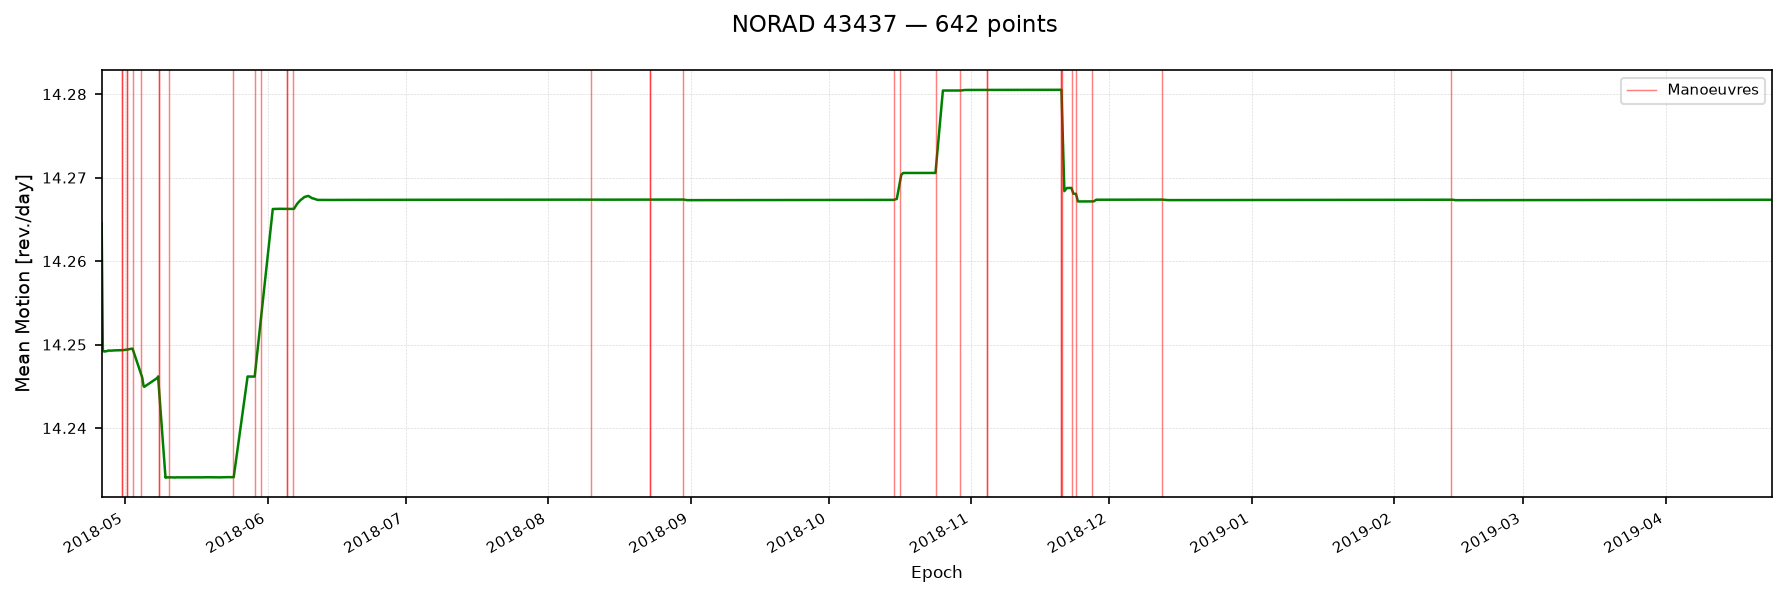
\includegraphics[width=0.48\textwidth]{figures/s3b_mean_motion.png}
\end{center}

\subsubsection{Envisat (NORAD 27386)}

\begin{center}
    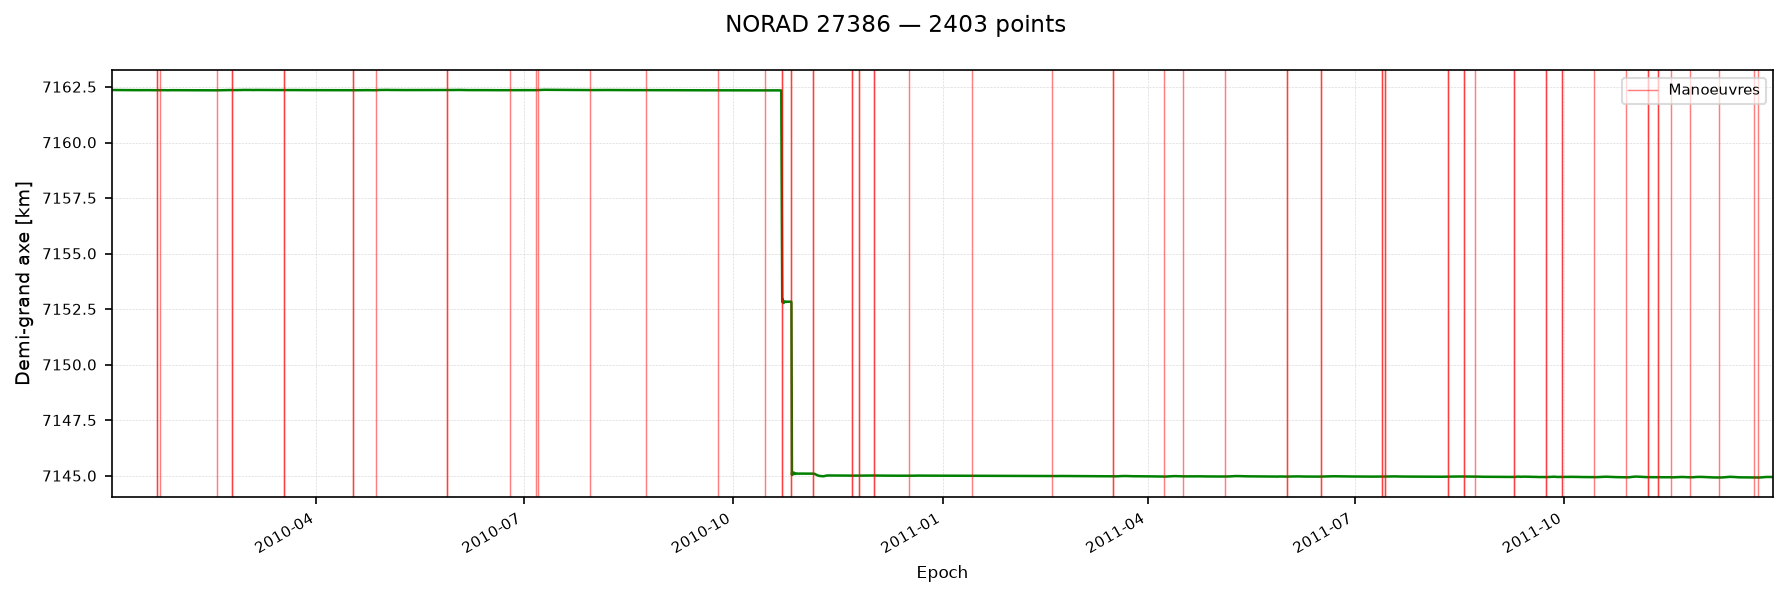
\includegraphics[width=0.48\textwidth]{figures/en1_sma.png}
    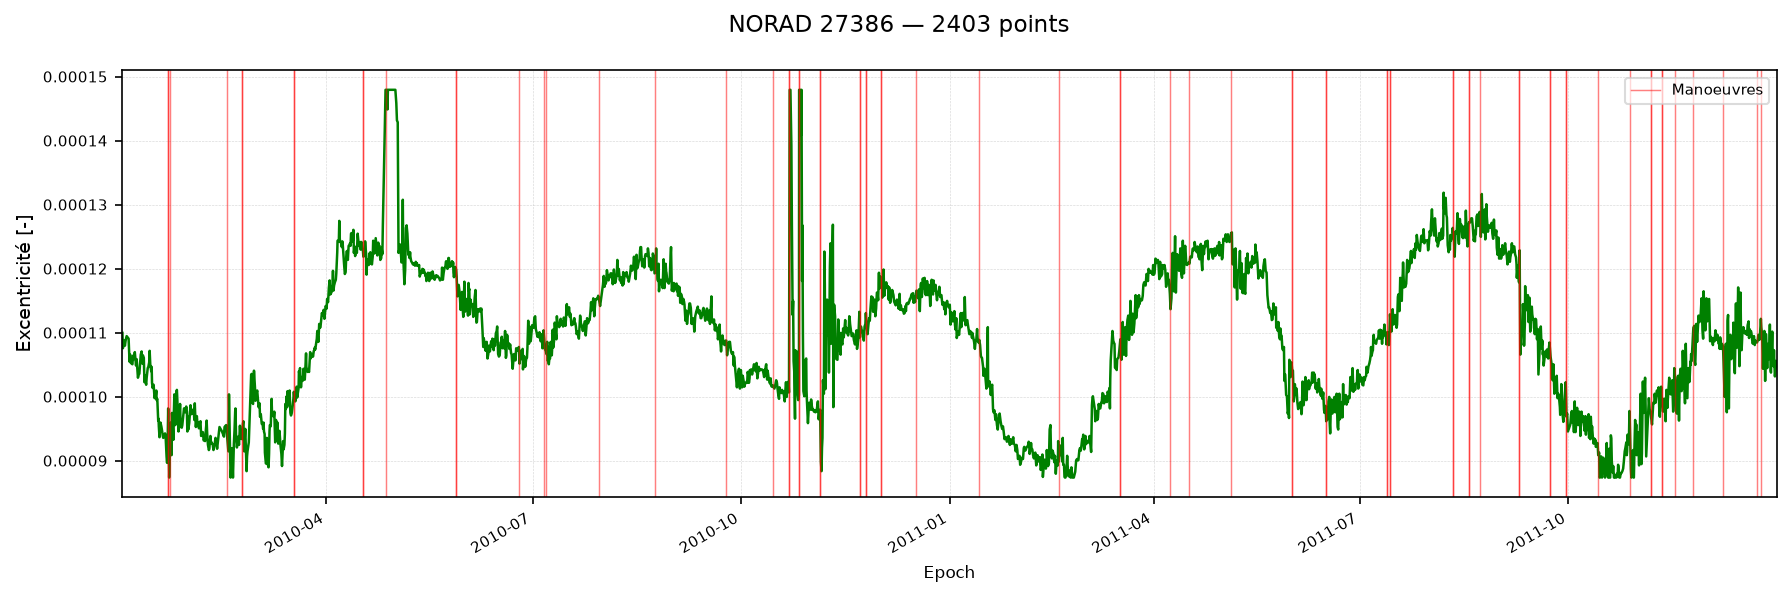
\includegraphics[width=0.48\textwidth]{figures/en1_eccentricity.png}
    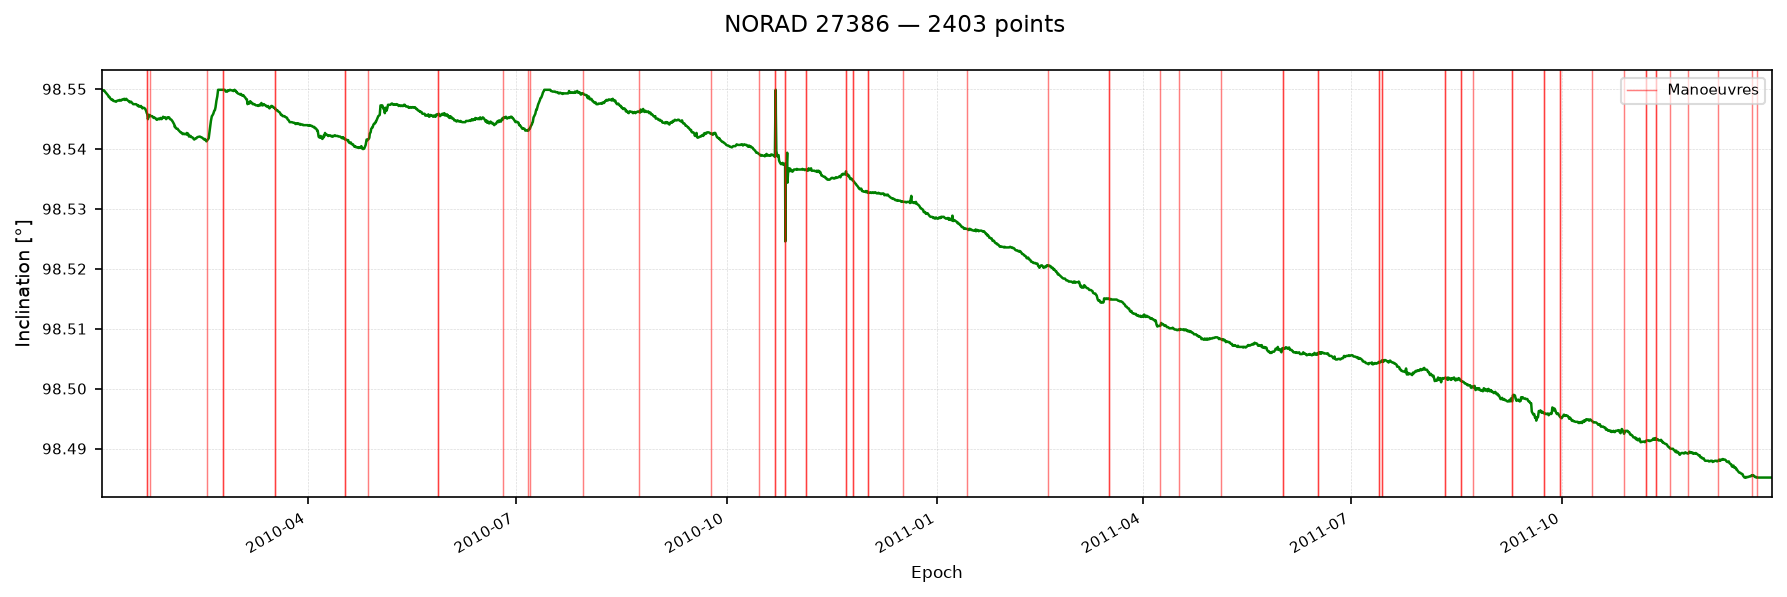
\includegraphics[width=0.48\textwidth]{figures/en1_inclination.png}
    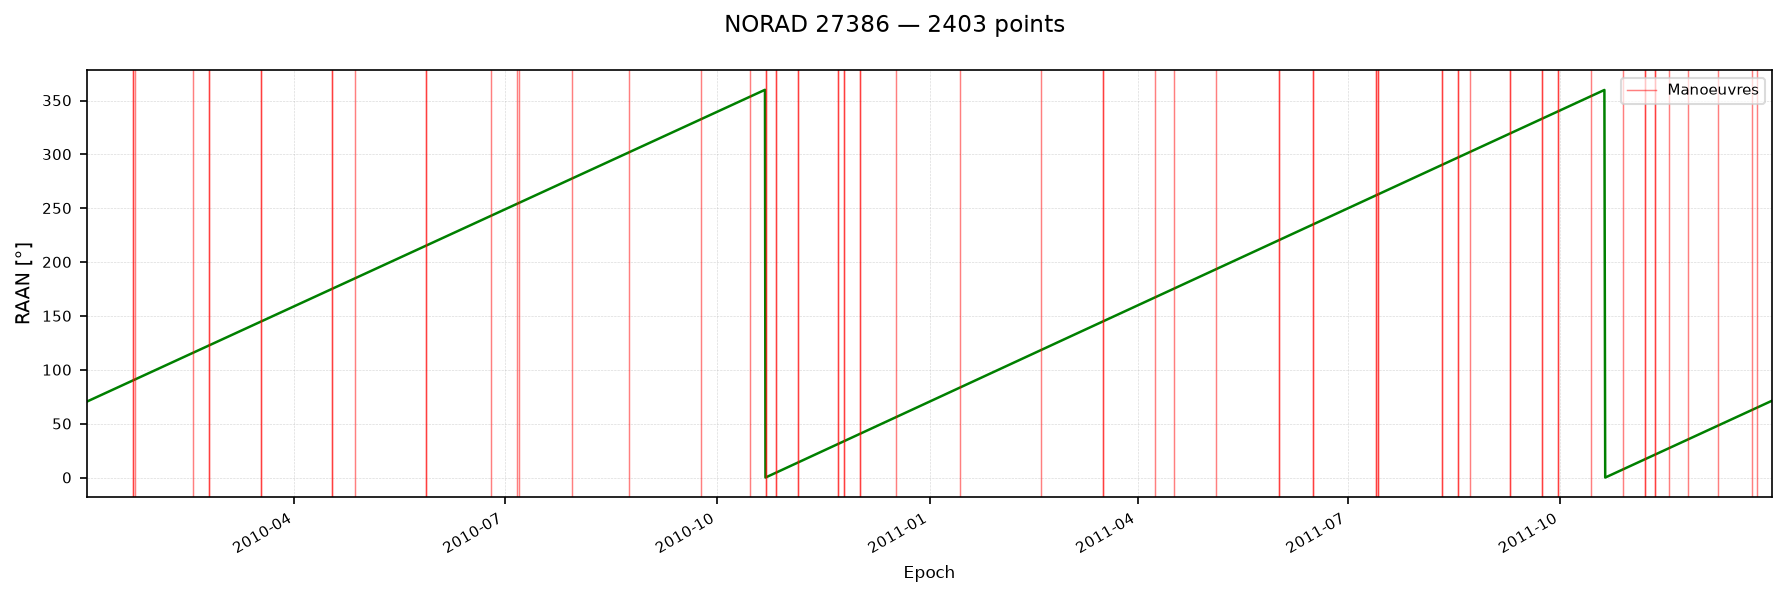
\includegraphics[width=0.48\textwidth]{figures/en1_raan.png}
    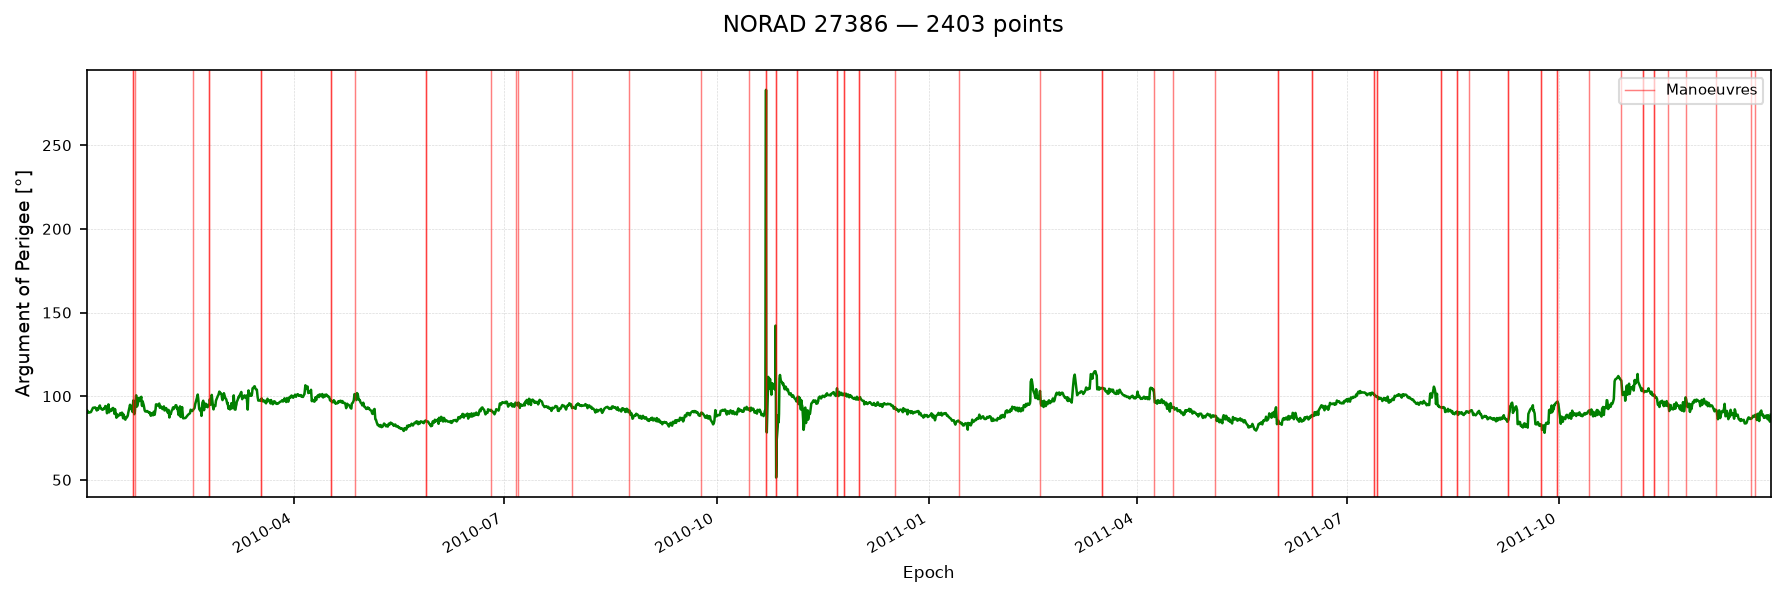
\includegraphics[width=0.48\textwidth]{figures/en1_arg_perigee.png}
    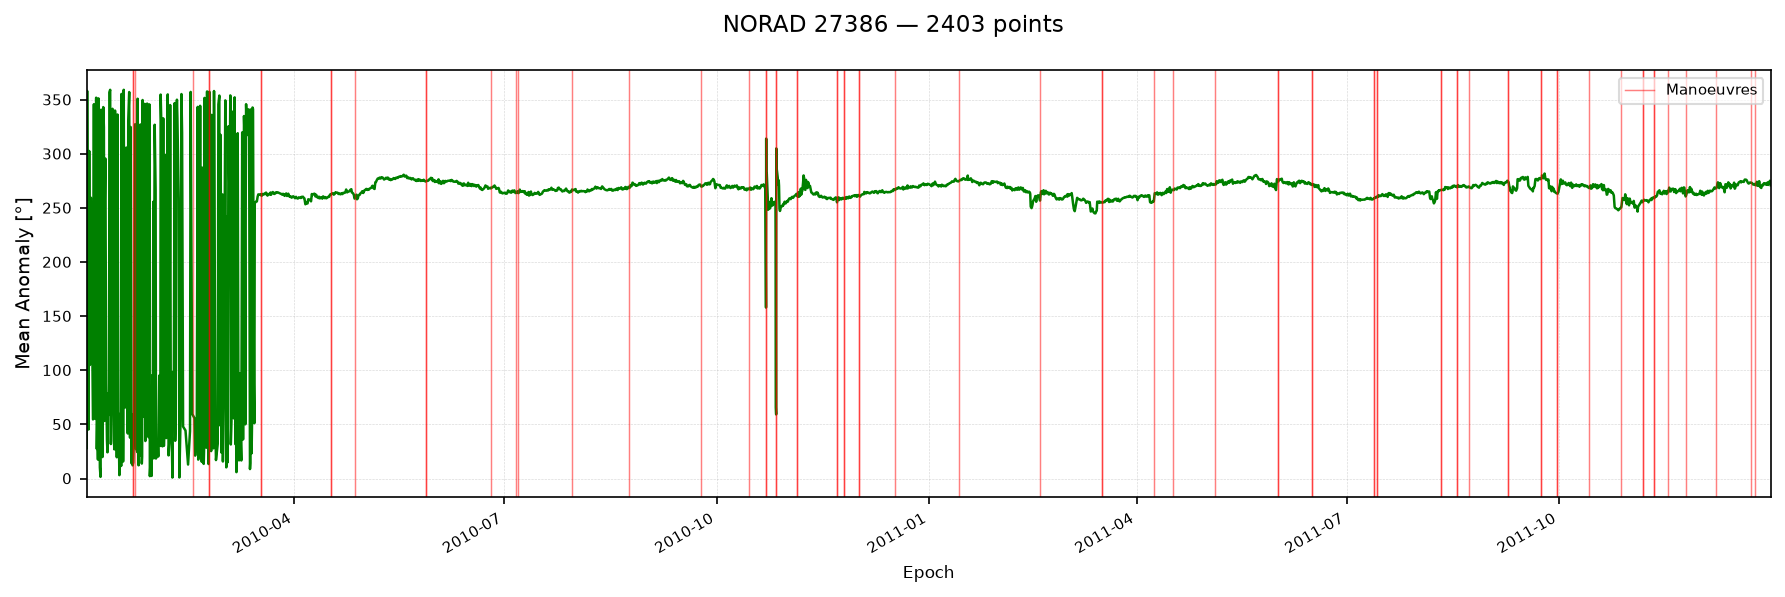
\includegraphics[width=0.48\textwidth]{figures/en1_mean_anomaly.png}
    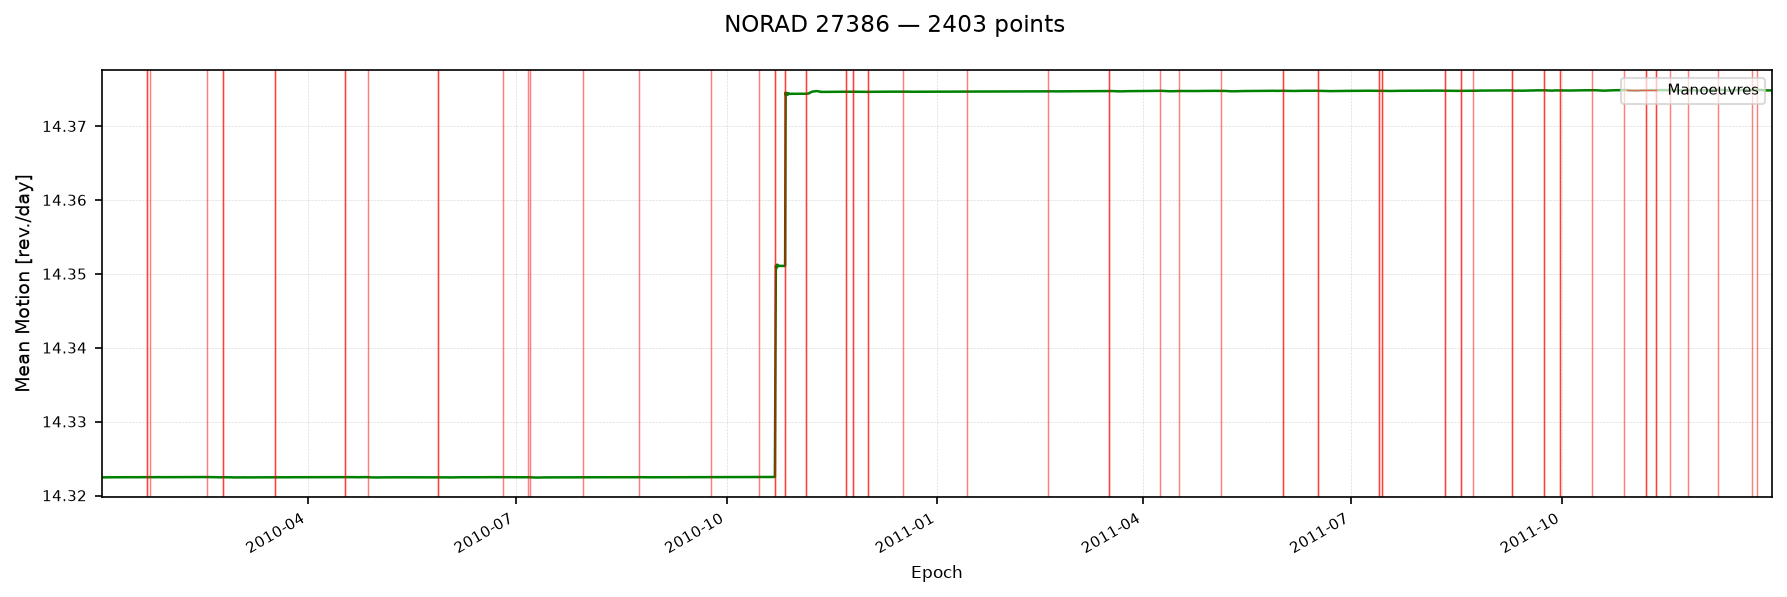
\includegraphics[width=0.48\textwidth]{figures/en1_mean_motion.png}
\end{center}

\subsubsection{CryoSat-2 (NORAD 36508)}

\begin{center}
    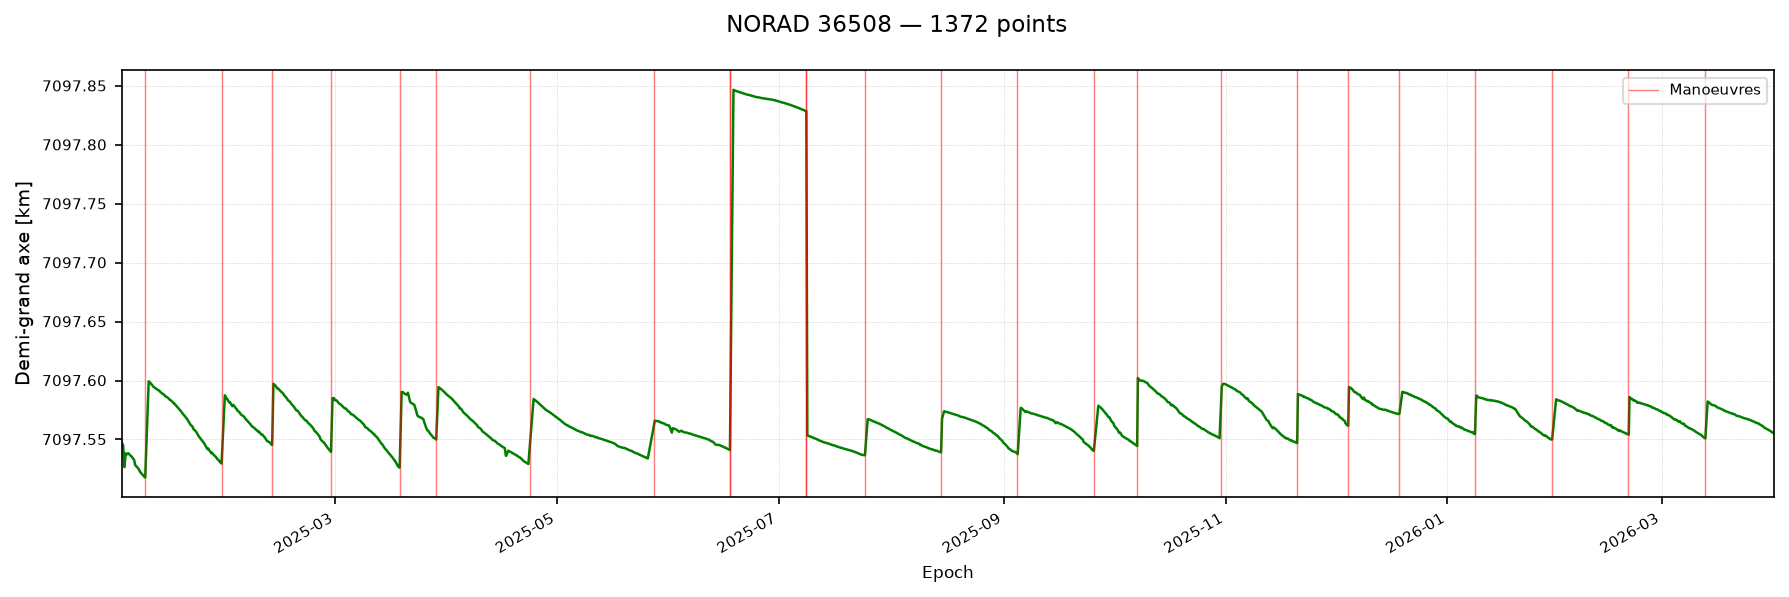
\includegraphics[width=0.48\textwidth]{figures/cs2_sma.png}
    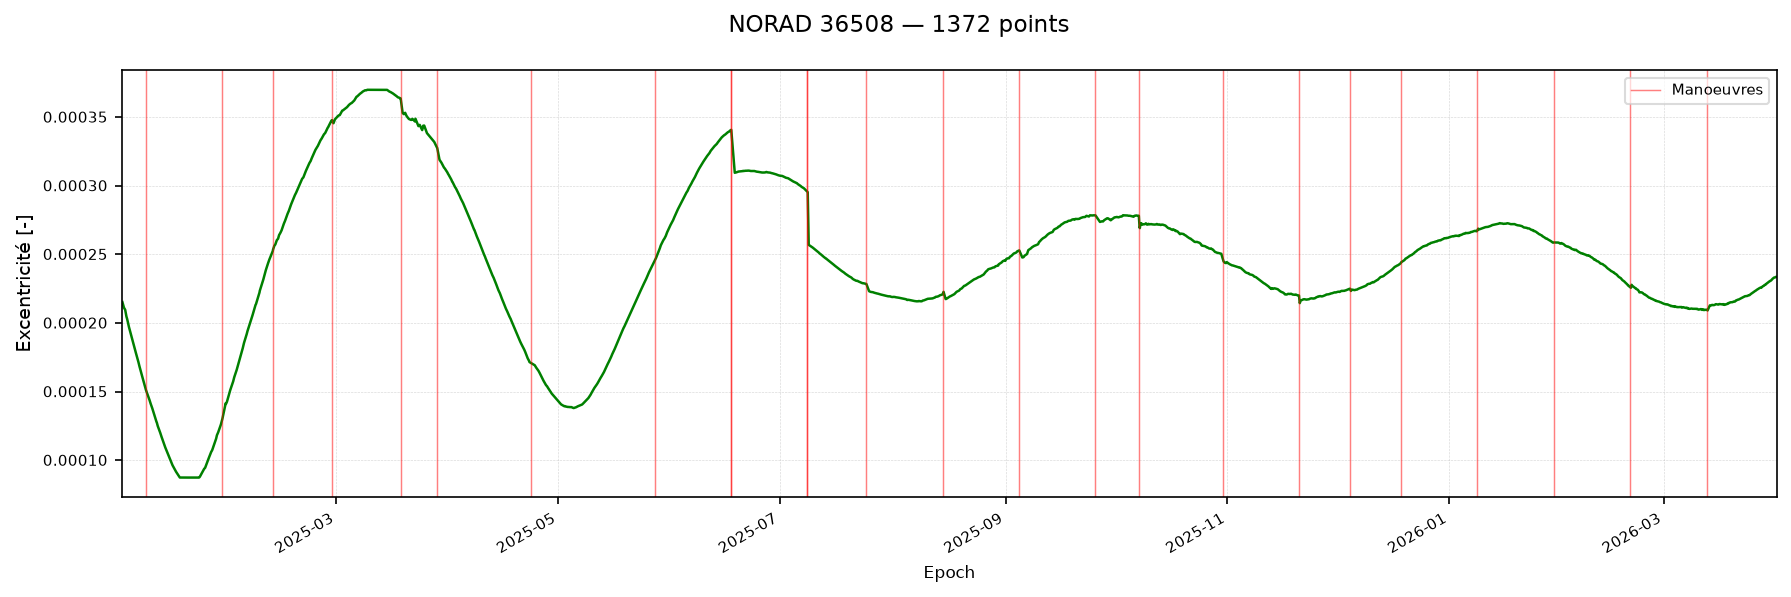
\includegraphics[width=0.48\textwidth]{figures/cs2_eccentricity.png}
    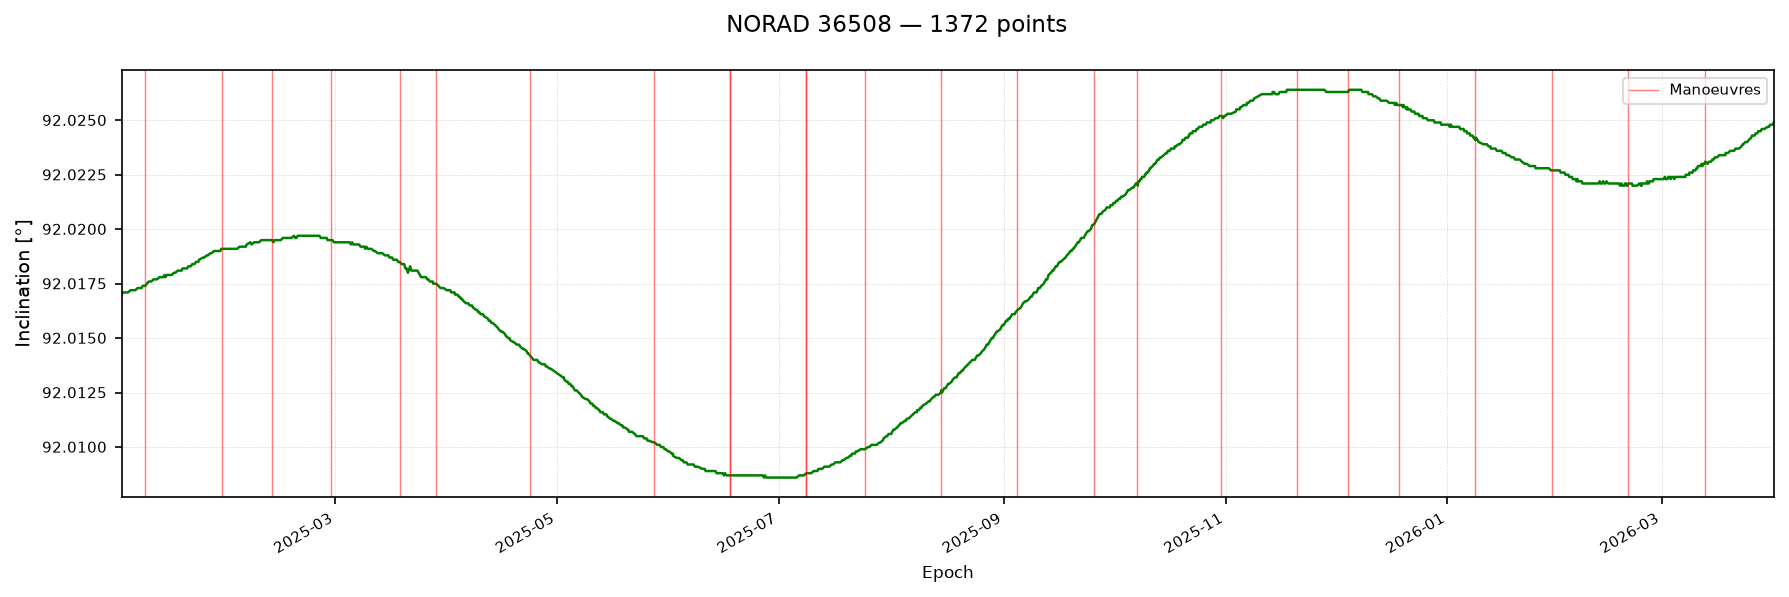
\includegraphics[width=0.48\textwidth]{figures/cs2_inclination.png}
    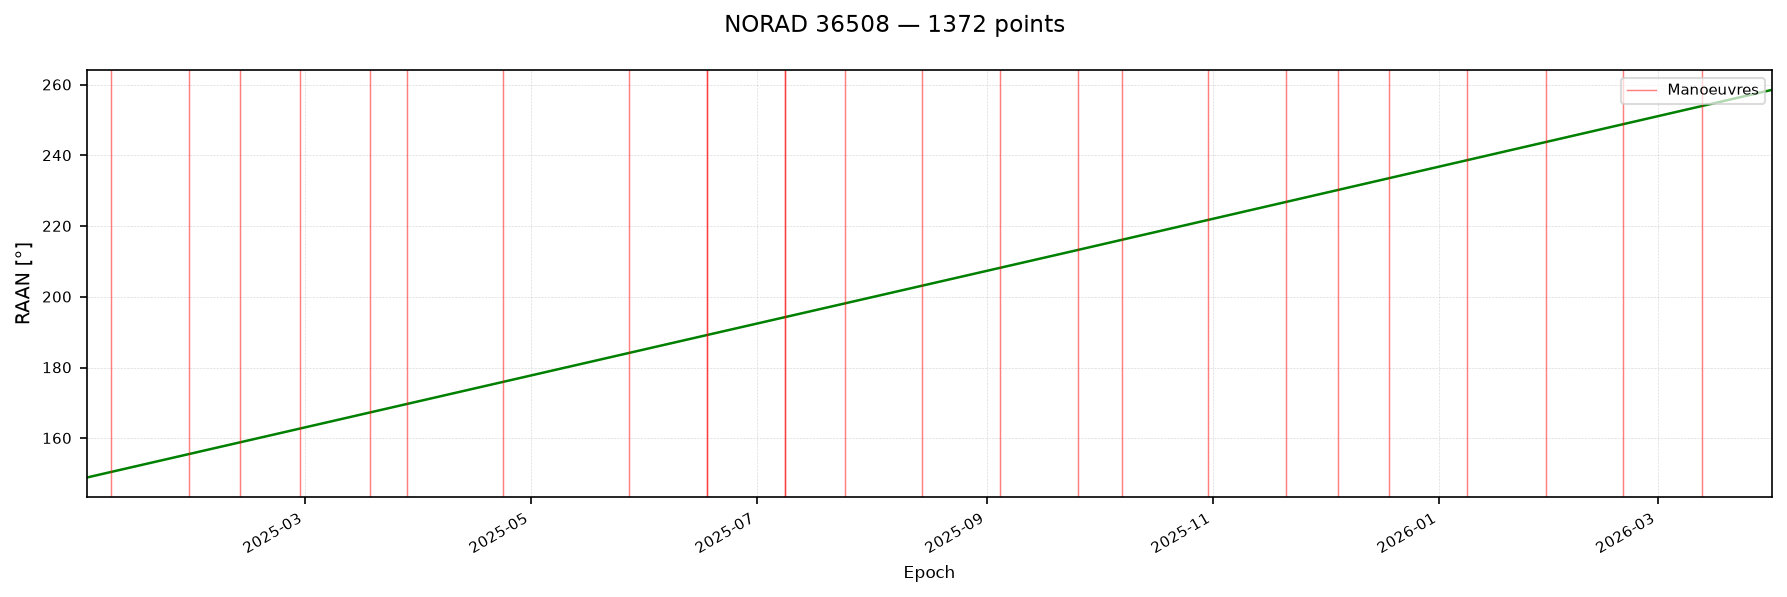
\includegraphics[width=0.48\textwidth]{figures/cs2_raan.png}
    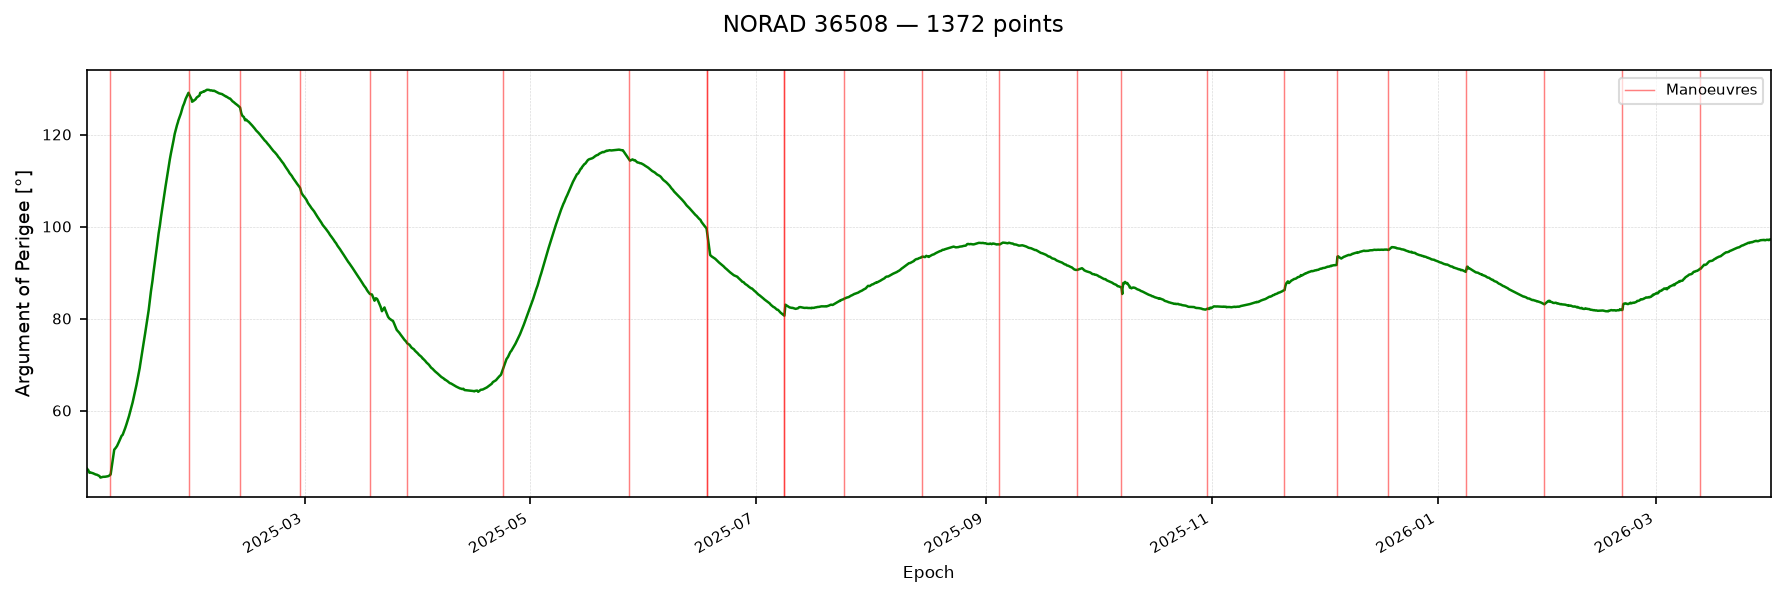
\includegraphics[width=0.48\textwidth]{figures/cs2_arg_perigee.png}
    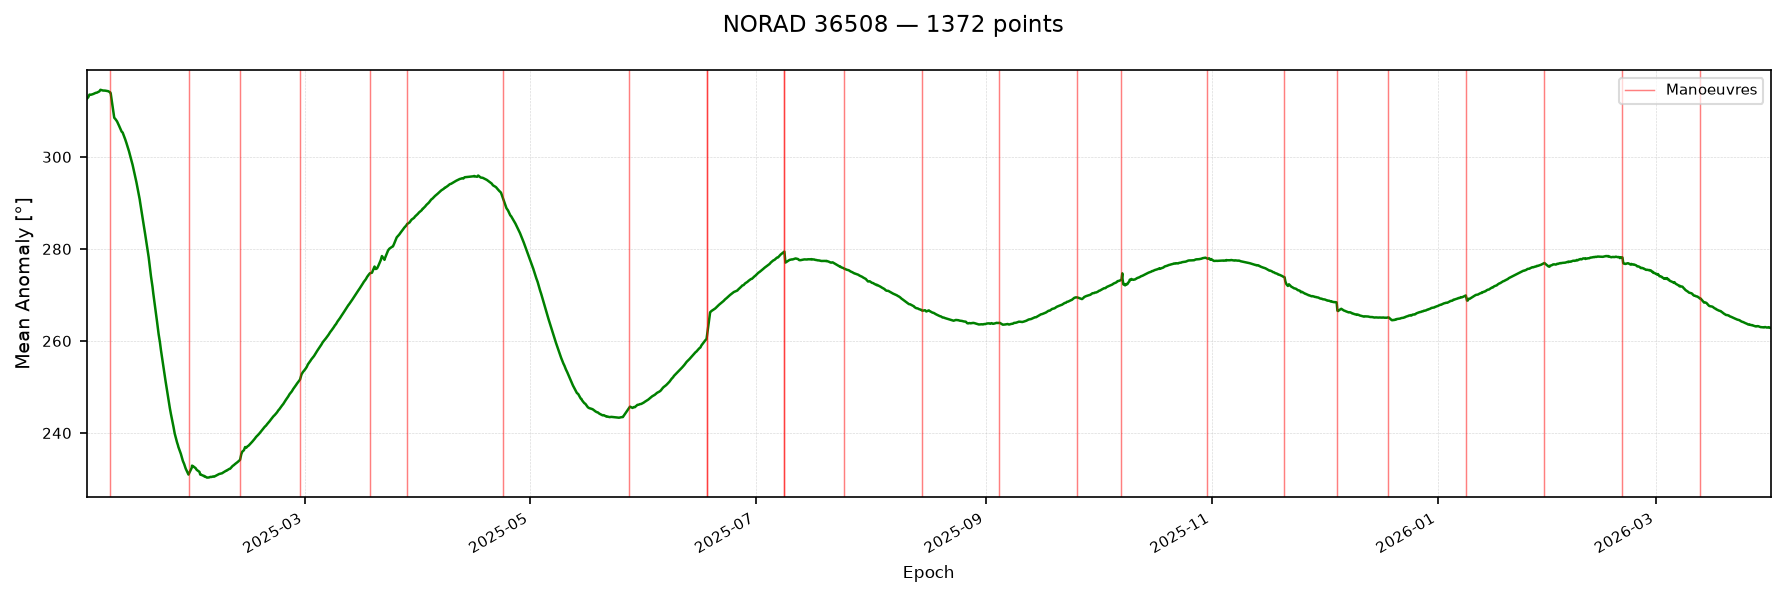
\includegraphics[width=0.48\textwidth]{figures/cs2_mean_anomaly.png}
    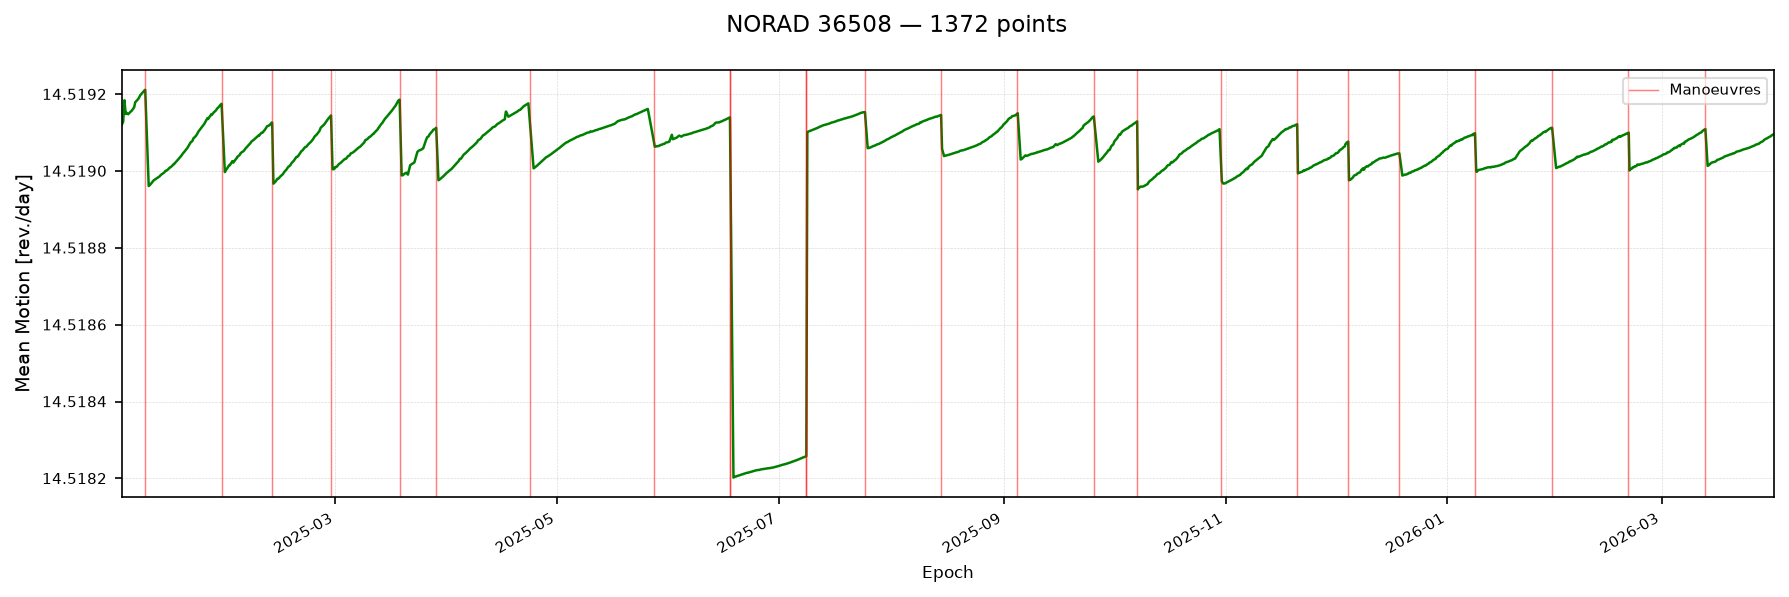
\includegraphics[width=0.48\textwidth]{figures/cs2_mean_motion.png}
\end{center}

\subsubsection{SARAL (NORAD 39086)}

\begin{center}
    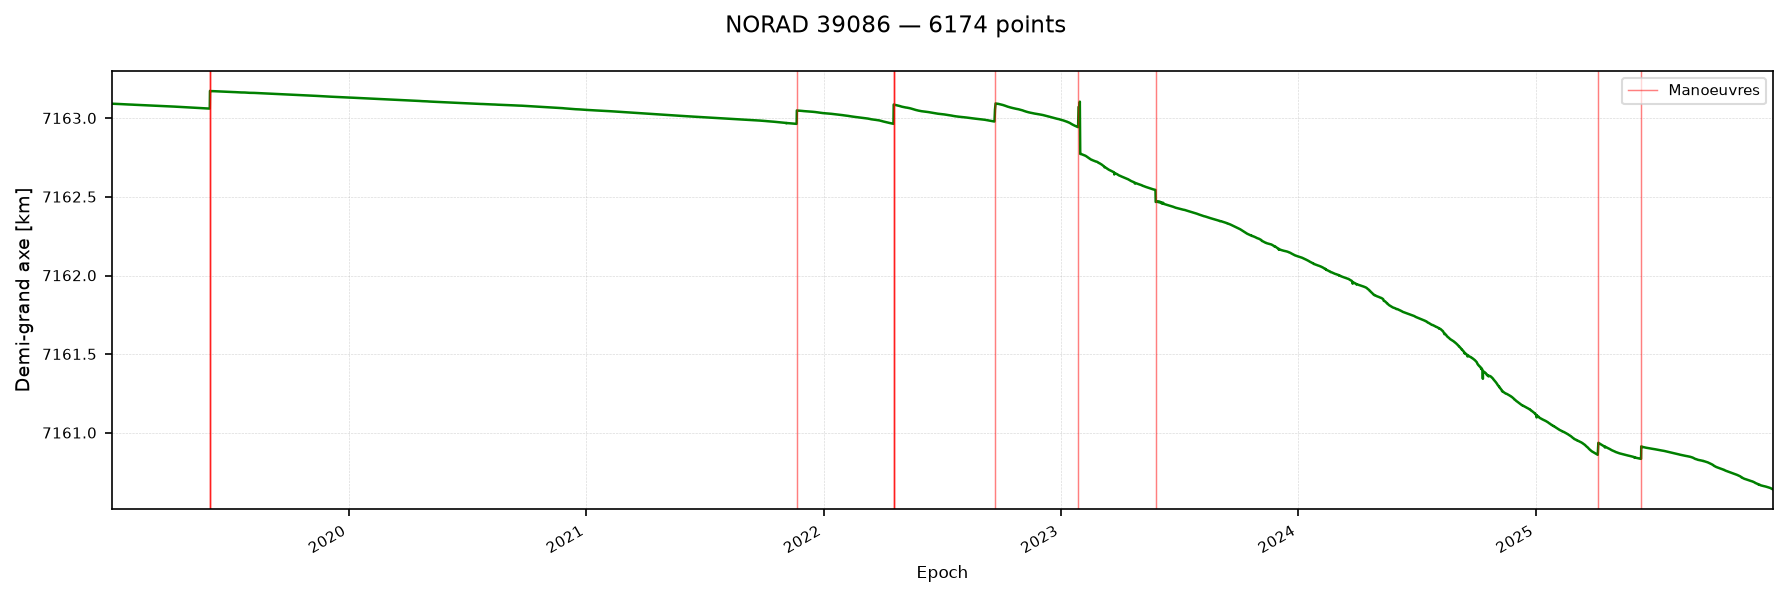
\includegraphics[width=0.48\textwidth]{figures/srl_sma.png}
    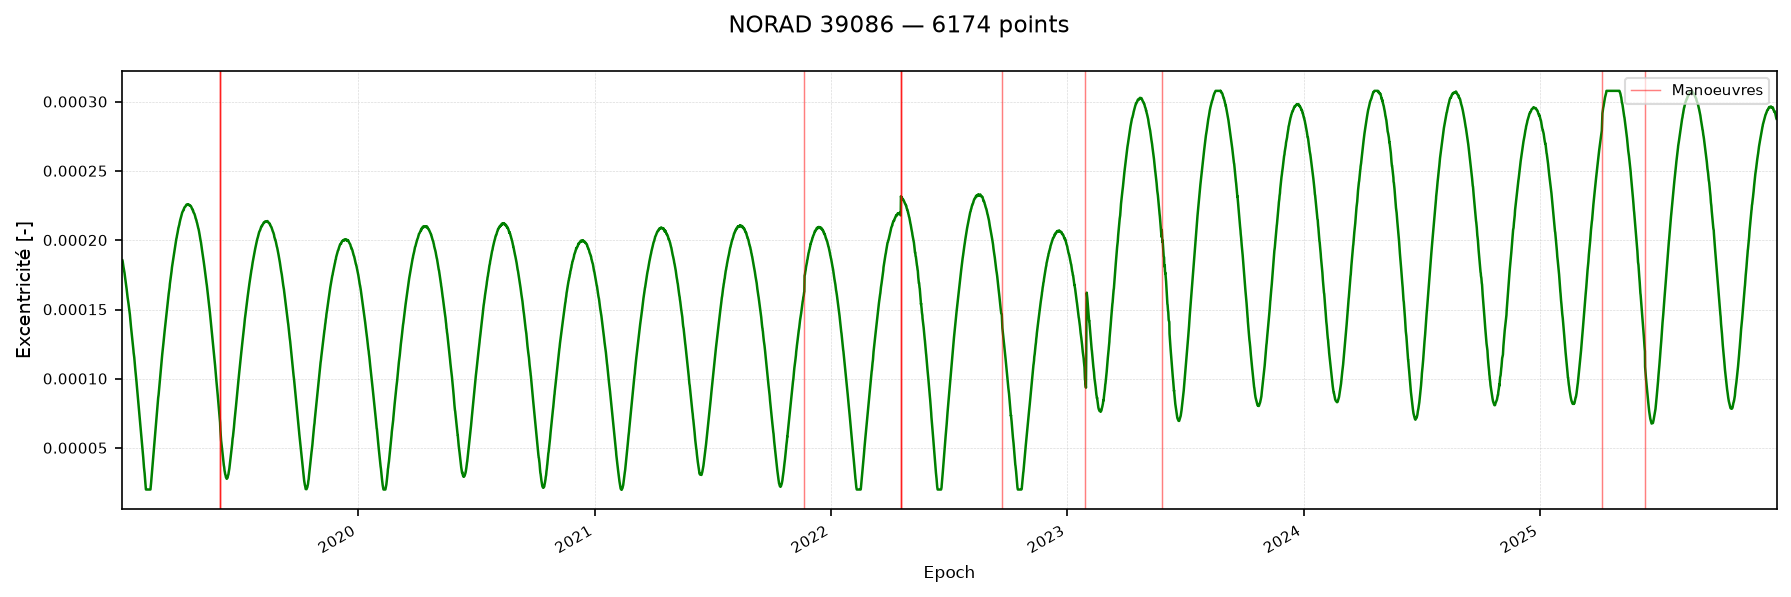
\includegraphics[width=0.48\textwidth]{figures/srl_eccentricity.png}
    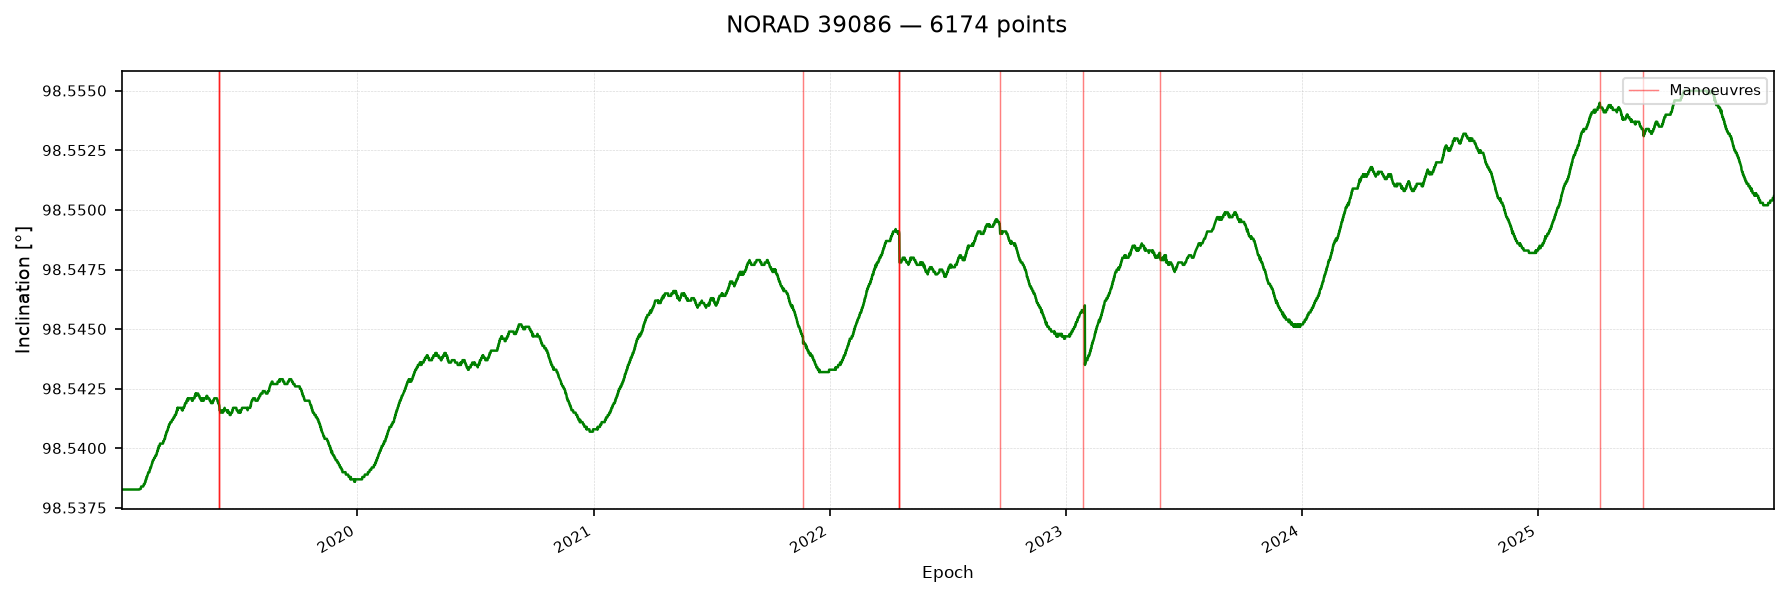
\includegraphics[width=0.48\textwidth]{figures/srl_inclination.png}
    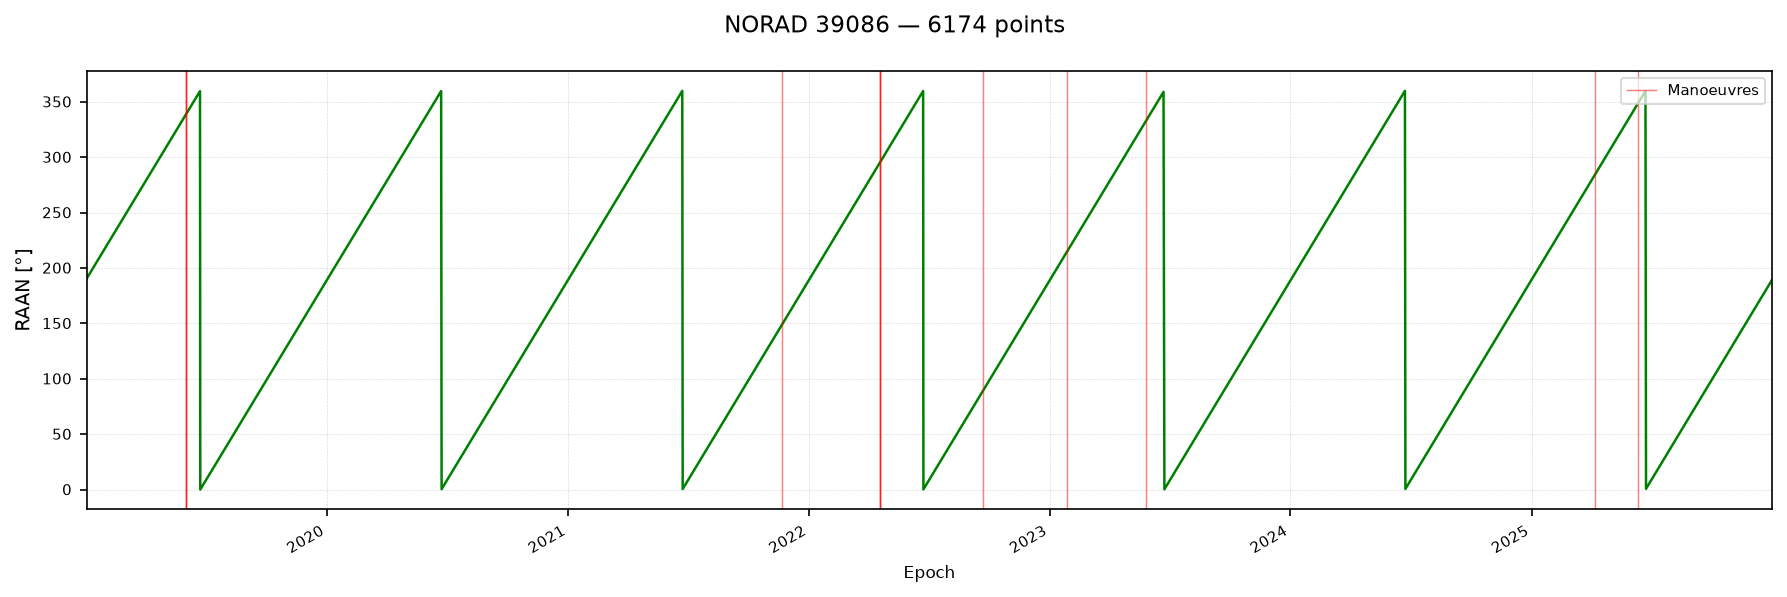
\includegraphics[width=0.48\textwidth]{figures/srl_raan.png}
    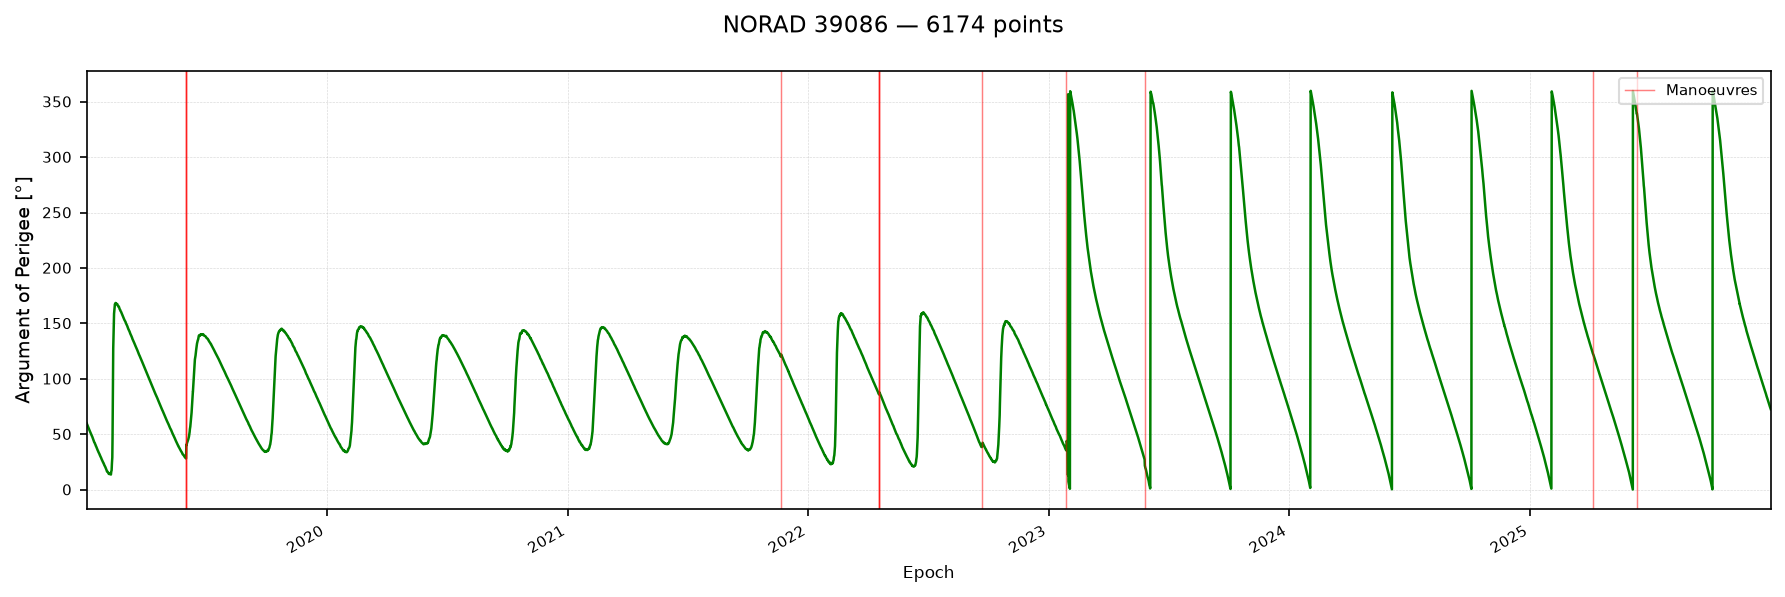
\includegraphics[width=0.48\textwidth]{figures/srl_arg_perigee.png}
    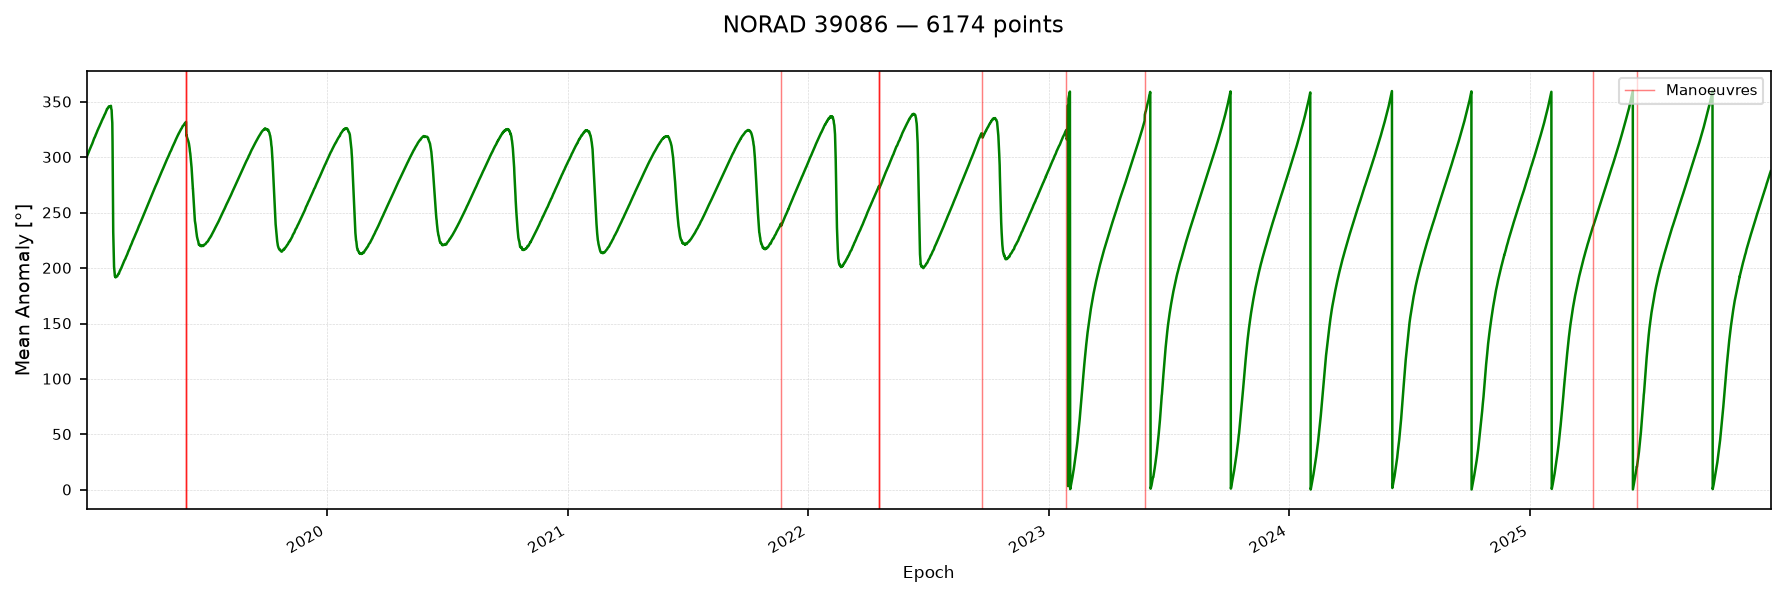
\includegraphics[width=0.48\textwidth]{figures/srl_mean_anomaly.png}
    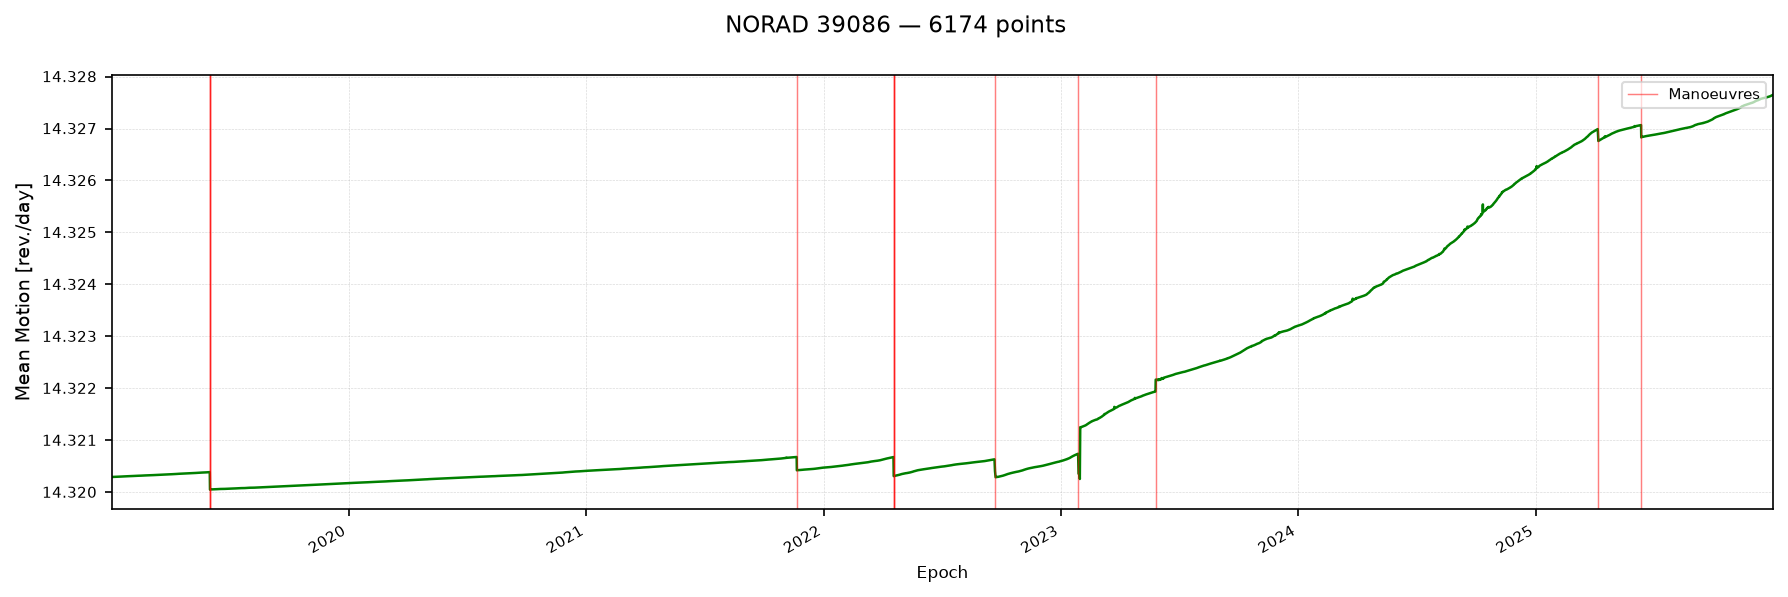
\includegraphics[width=0.48\textwidth]{figures/srl_mean_motion.png}
\end{center}

Certaines manoeuvres sont clairement visibles à l'oeil nu sur les séries des paramètres orbitaux, tandis que d'autres ne se détectent pas via un simple regard non expert.
Le demi-grand axe est souvent le meilleur moyen de détecter des manoeuvres visuellement, d'où la pertinence de mettre en place des algorithmes de détection basés sur cette métrique.

\subsubsection{Vérification de la loi de Gauss in-plane}

Une variation du demi-grand axe $a$ est liée à une variation de la vitesse transverse $\Delta v_u$. Dans le cas d'une orbite quasi-circulaire (ici $e \sim 10^{-4}$), on a grossièrement :
$$
\Delta a = \dfrac{2}{n} \Delta v_u
$$

On teste cette loi en comparant, pour chaque satellite, $\Delta a_{\text{approx}} \sim \dot a_{\text{Kalman}} \, \Delta t$, où $\dot a$ est la dérivée du demi-grand axe estimée par le filtre de Kalman, à $\Delta a_{\text{théorique}} = \dfrac{2}{n} \Delta v_{u,\text{mesuré}}$ calculé à partir des $\Delta v$ transverses fournis par l'ILRS.

\begin{center}
    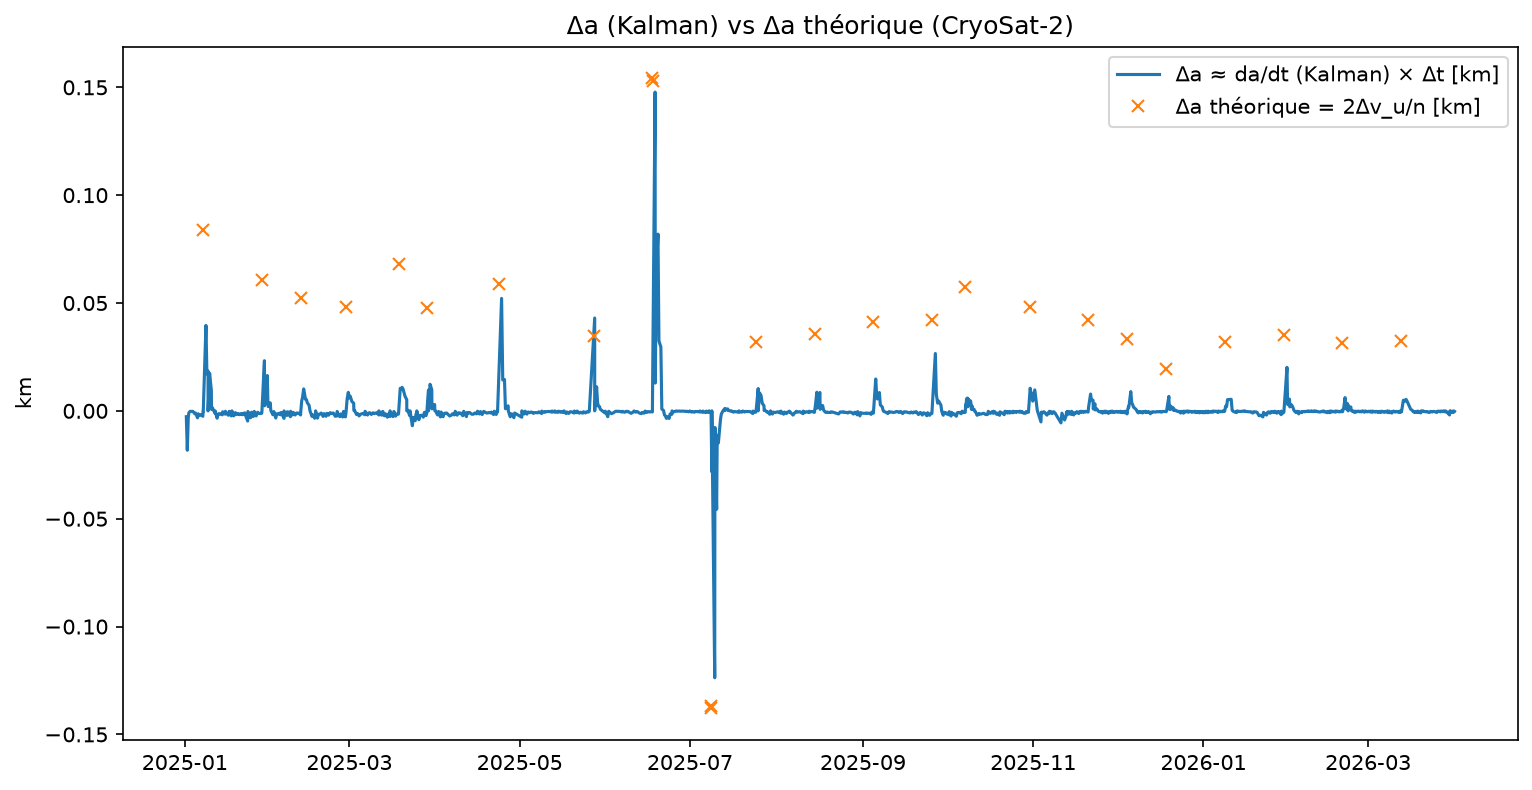
\includegraphics[width=0.85\textwidth]{figures/cs2_delta_a_kalman_vs_theorique.png}
\end{center}
\begin{center}
    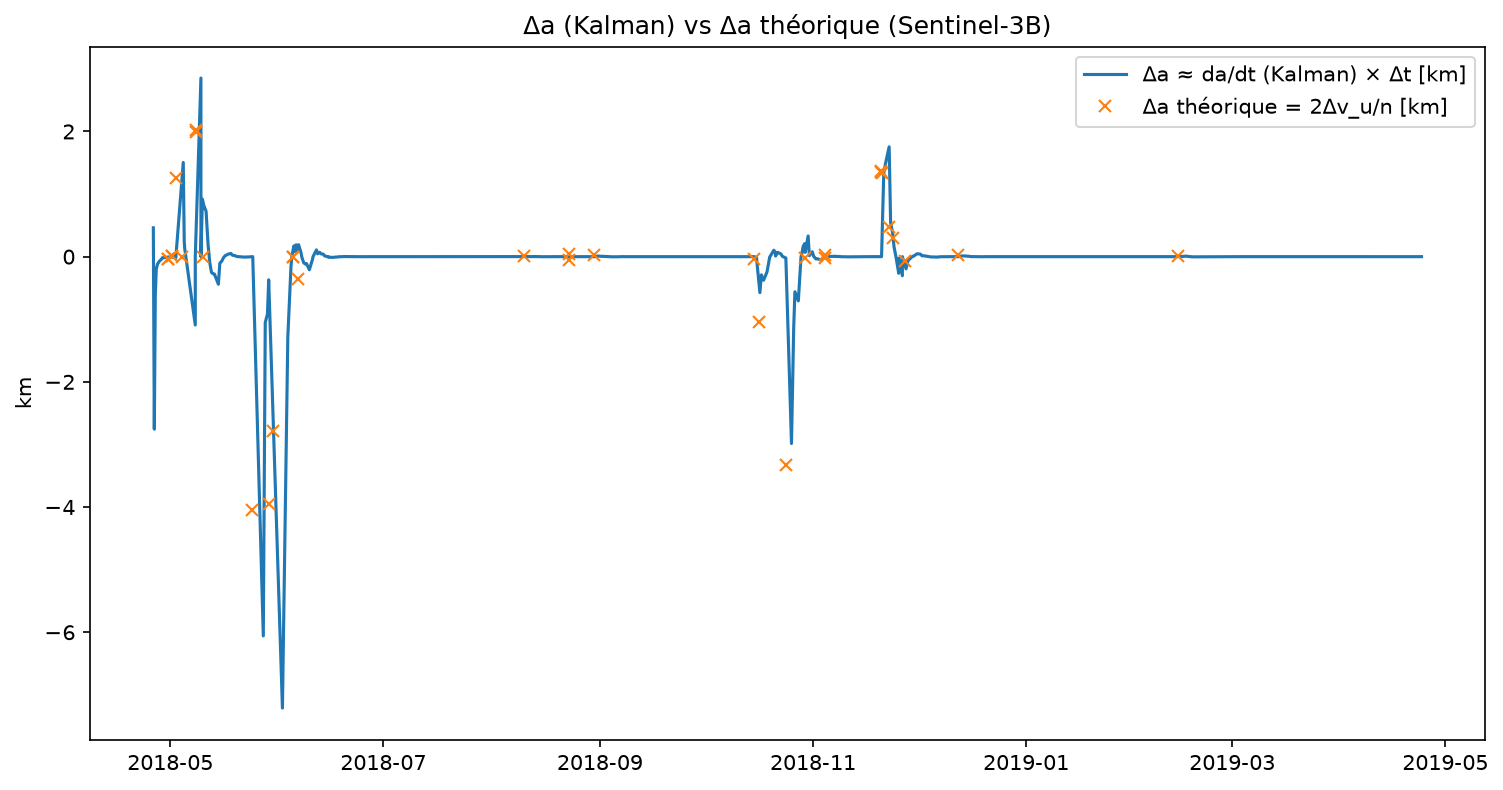
\includegraphics[width=0.85\textwidth]{figures/s3b_delta_a_kalman_vs_theorique.png}
\end{center}

La loi théorique, dérivée des équations de Gauss dans le cas d'orbite quasi-circulaire, est bien vérifiée : les deux quantités sont du même ordre de grandeur et les pics coïncident avec les manoeuvres.
L'écart entre les pics et les valeurs théoriques de $\Delta a$ s'explique par le choix, pour l'instant plus ou moins arbitraire, des paramètres du filtre de Kalman, notamment $r$, l'incertitude de mesure aléatoire sur le demi-grand axe, qui fait varier plus ou moins l'intensité des pics.

\subsubsection{Typologie des manoeuvres : composantes de $\Delta v$}

Les manoeuvres résultant d'une variation $\Delta v_u$ transverse correspondent à des manoeuvres in-plane de replacement du satellite.
On peut quantifier cela en remontant directement à $\Delta v_u$ depuis une mesure d'une variation $\Delta a$, avec une méthode de détection de manoeuvres bien calibrée.
Pour déterminer si les manoeuvres sont purement in-plane, on trace, pour chaque manoeuvre, les trois composantes de la variation de vitesse.

\begin{center}
    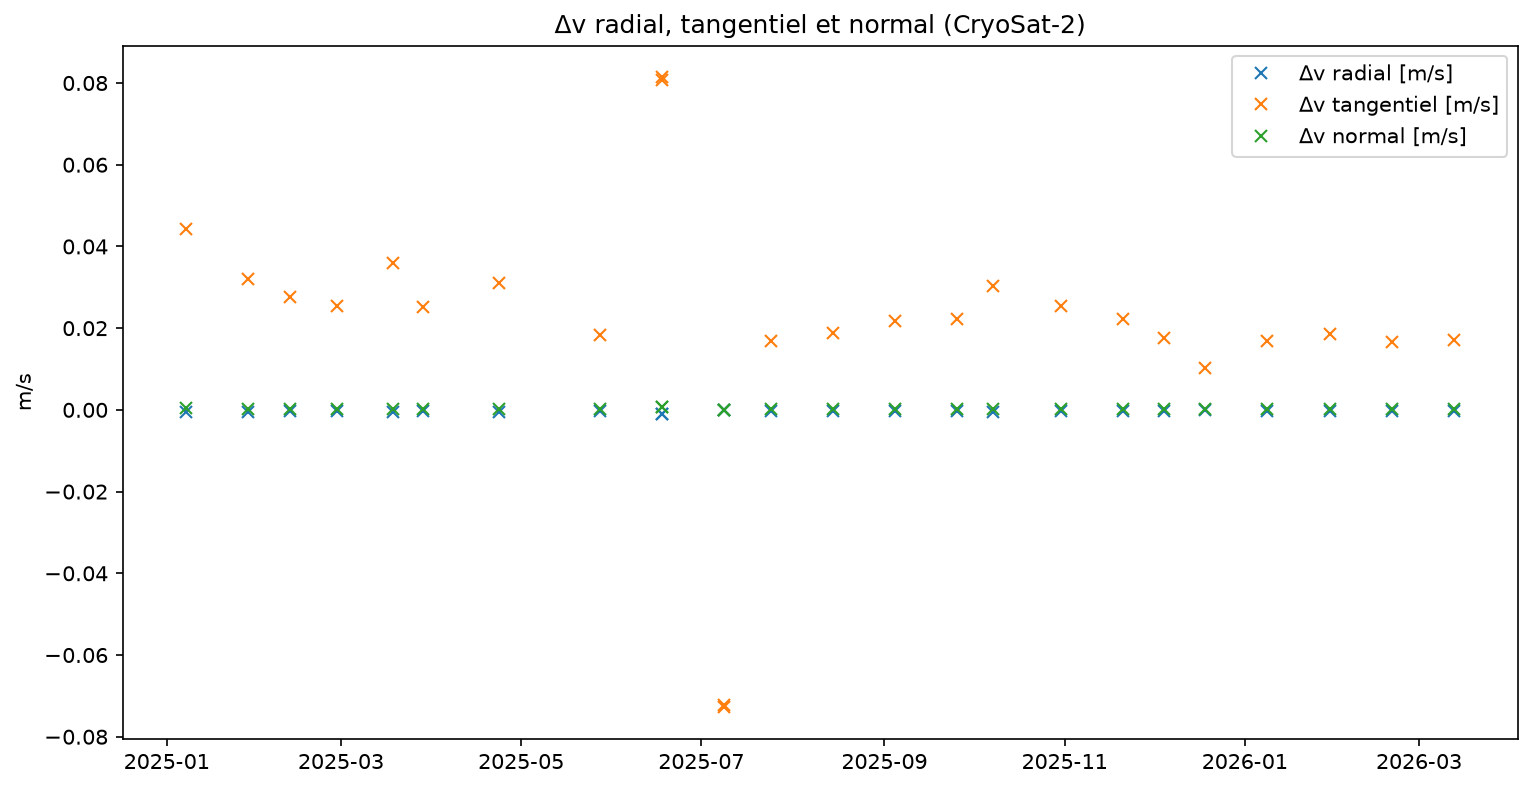
\includegraphics[width=0.85\textwidth]{figures/cs2_dv_composantes.png}
\end{center}
\begin{center}
    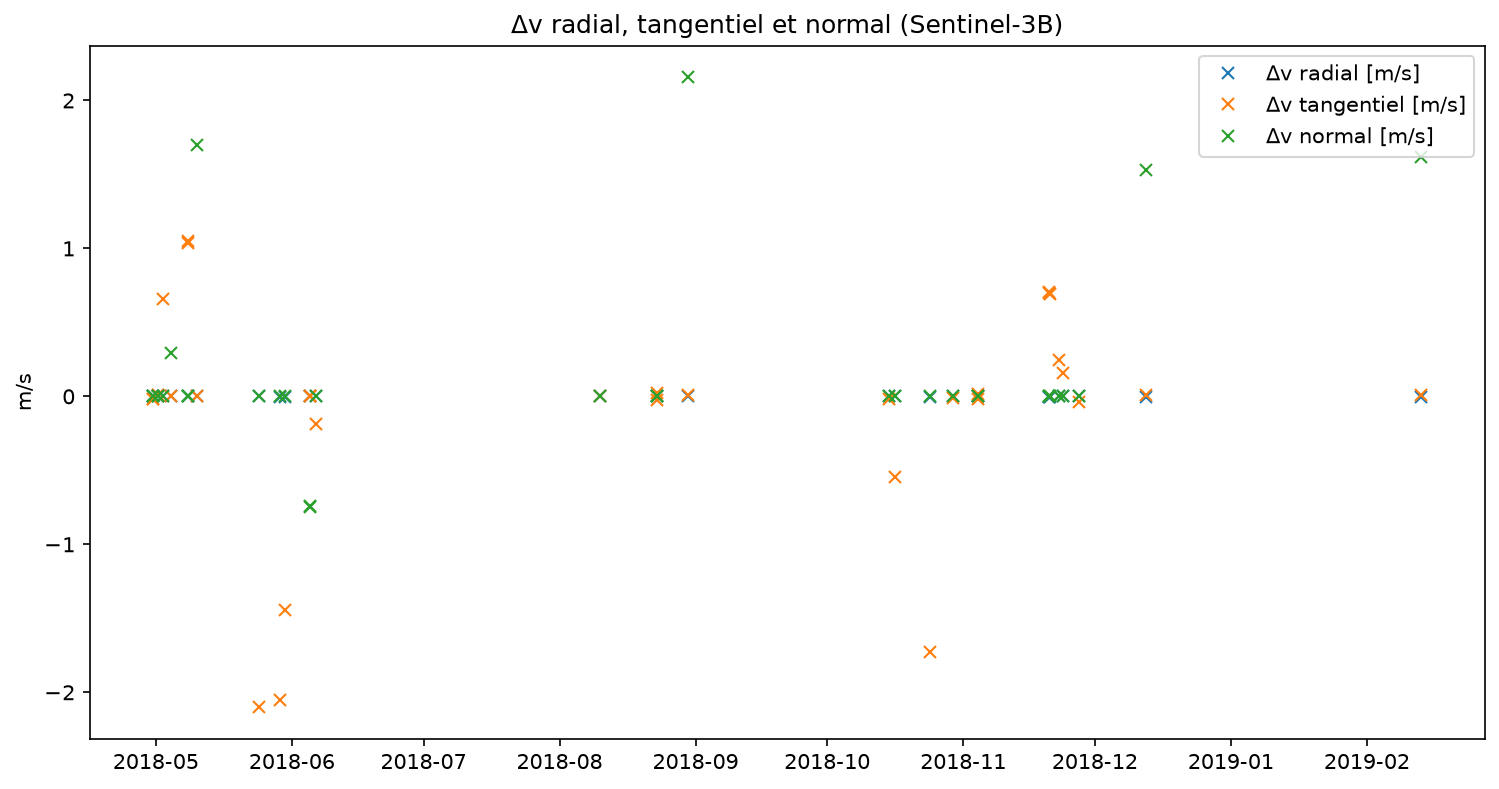
\includegraphics[width=0.85\textwidth]{figures/s3b_dv_composantes.png}
\end{center}

Pour CryoSat-2, les manoeuvres sont purement transverses, donc purement in-plane.
Pour Sentinel-3B en revanche, un certain nombre de manoeuvres possèdent une composante normale importante : ces variations de vitesse normale créent des manoeuvres out-plane.

\subsubsection{Canal d'observation des manoeuvres out-plane}

Les manoeuvres out-plane se traduisent a priori par des variations de l'inclinaison et de la RAAN. L'équation de Gauss reliant une perturbation normale de la vitesse aux variations de $i$ et $\Omega$ s'écrit :
$$
\Delta i = \dfrac{r}{n a^2} \cos(\omega + \nu) \, \Delta v_n \quad ; \quad \Delta \Omega = \dfrac{r}{n a^2} \dfrac{\sin(\omega + \nu)}{\sin i} \, \Delta v_n
$$
où $n = \dfrac{2\pi}{T}$ est le mouvement moyen, $r \sim a$ la distance du foyer au satellite et $\nu$ l'anomalie vraie.

Cependant, on ne voit ici aucun effet des manoeuvres sur la RAAN.
On est dans le cas d'une orbite quasi-polaire ($i \sim 98 \degres $) : la dérive de $\Omega$ liée au terme de perturbation du champ gravitationnel l'emporte.
En coordonnées sphériques, on a au premier ordre :
$$
U_{\text{Terre}}(r, \lambda, \theta) = U_0 + U_{J_2} = -\dfrac{\mu}{r}\left( 1 - \dfrac{J_2}{2} \left(\dfrac{R_T}{r}\right)^2 (3 \sin^2 \lambda - 1)\right)
$$
et le terme $U_{J_2}$ induit une dérive de $\Omega$ :
$$
\dot{\Omega}_{J_2} = -\dfrac{3}{2} J_2 \left(\dfrac{R_T}{r}\right)^2 n \cos i \sim 1 \degres /\text{jour}
$$
tandis que les variations dues aux manoeuvres sont de l'ordre de $0{,}01 \degres /\text{jour}$.

\textbf{Remarque.}
Tout cela n'est plus vrai pour des orbites à faible inclinaison : si $i \sim 0 \degres $, $\Omega$ varie en $\dfrac{1}{\sin i}$ et devient un canal d'observation valable (la discontinuité des paramètres angulaires nécessite alors d'ailleurs un changement de coordonnées vers les coordonnées équinoxiales).

Pour analyser les manoeuvres out-plane, on se base donc sur les variations de l'inclinaison, et on teste la loi de Gauss comme précédemment pour le demi-grand axe, en appliquant cette fois le filtre de Kalman à l'inclinaison (avec un bruit de mesure $r$ adapté, beaucoup plus petit que pour $a$) :

\begin{center}
    
\includegraphics[width=0.85\textwidth]{figures/s3b_delta_i_kalman_vs_theorique.png}
\end{center}


\subsubsection{Performances de la détection sur les satellites ILRS}

On ne s'interesse qu'à notre algorithme déterministe LKF d'ordre 1 ou 2. 
La difficulté lorsque l'on veut appliquer une détection statistique avec une filtration Kalman, c'est la dépendance du filtre aux paramètres initiaux, qui implique de faire du seuillage au cas par cas.
Pour pallier cette difficulté, on raisonne de la manière suivante : on observe une métrique unique, les résidus (qui sont les prédictions du filtre - observation) normalisés (NIS $\varepsilon $), et dont les anomalies dépendent des paramètres du filtre, et qui suivent une loi connue.
Un seuil statistique unique est appliqué aux NIS (à savoir un quantile d'ordre 0.997 de cette loi). Ce qu'on l'on va optimiser en revanche, ce sont les paramètres initiaux du filtres. 

On va ici donc utiliser cette méthode pour les 4 satellites dont on connait l'historique des manoeuvres vraies.

On introduit la fonction suivante qui mesure la performance du filtre :

$$
F_1 = \dfrac{2 \text{Pr}  * \text{Re}}{\text{Pr}  + \text{Re}}
$$

où 

$$
\text{Pr} = \dfrac{n_{det}}{n_{det} + n_{false}} \quad \text{Re} = \dfrac{n_{det}}{n_{det} + n_{missed}}
$$
Le but est d'optimiser cette métrique en fonction des paramères $r, var_Q, P0$ du filtre Kalman d'ordre 1 ou 2.
Problème : cette métrique est non régulière (constante par morceaux). 
On va donc la régulariser via un produit de convolution avec un noyau gaussien.

Supposons donc que l'on dispose (en jours par rapport à $t_0$) de $t_i$ des dates vraies de manoeuvres et $\tilde{t_i}$ des dates prédites de manoeuvres par filtrage des résidus du paramètre considéré (demi-grand axe, inclinaison, perigé, ...), ainsi que d'un score $s_i$ de la détection. Par exemple 
$$ 
s_i = | \varepsilon (\tilde{t_i}) - \text{seuil} | 
$$ 
Avec $\text{seuil} = quantile(\chi ^2(1), \alpha)$. 
On rappelle que $ \varepsilon \sim \chi ^ 2 (1) $ en l'absence de manoeuvres.

On introduit alors $ \sigma$ et $\beta$, deux paramètres de lissage.

$$
w_{ij} = e^{-\dfrac{(t_i - \tilde{t_j})^2}{2\sigma ^2}} \in \mathbb{R}^{n*n}
$$
matrice de poids de correspondance temporelle.
$$
p_j = \text{sigmoid}(\dfrac{s_j - seuil}{\beta}) \in \mathbb{R}^n 
$$
vecteur de probabilité de détection. 

Ainsi, les métriques lissées deviennent : 
$$
\tilde{\text{Pr}} = \dfrac{1}{n} \sum_{i = 1}^n \text{max}_j(w_{ij} p_j) \quad \tilde{\text{Re}} = \sum_{i = 1}^n p_i \text{max}_j(w_{ij})
$$
Puis : 
$$
\tilde{F_1}(X) = \dfrac{2 \tilde{\text{Pr}}  * \tilde{\text{Re}}}{\tilde{\text{Pr}}  + \tilde{\text{Re}}} \in \mathcal{C}^1 (\mathbb{R}^d, \mathbb{R})
$$
avec $X$ le vecteur des paramètres
 
On représente la métrique $F1$ brute ainsi que la métrique lissée pour les 4 satellites, en fonction du paramètre $r$ du filtre (représente l'incertitude sur la mesure du paramètre)
\begin{center}
    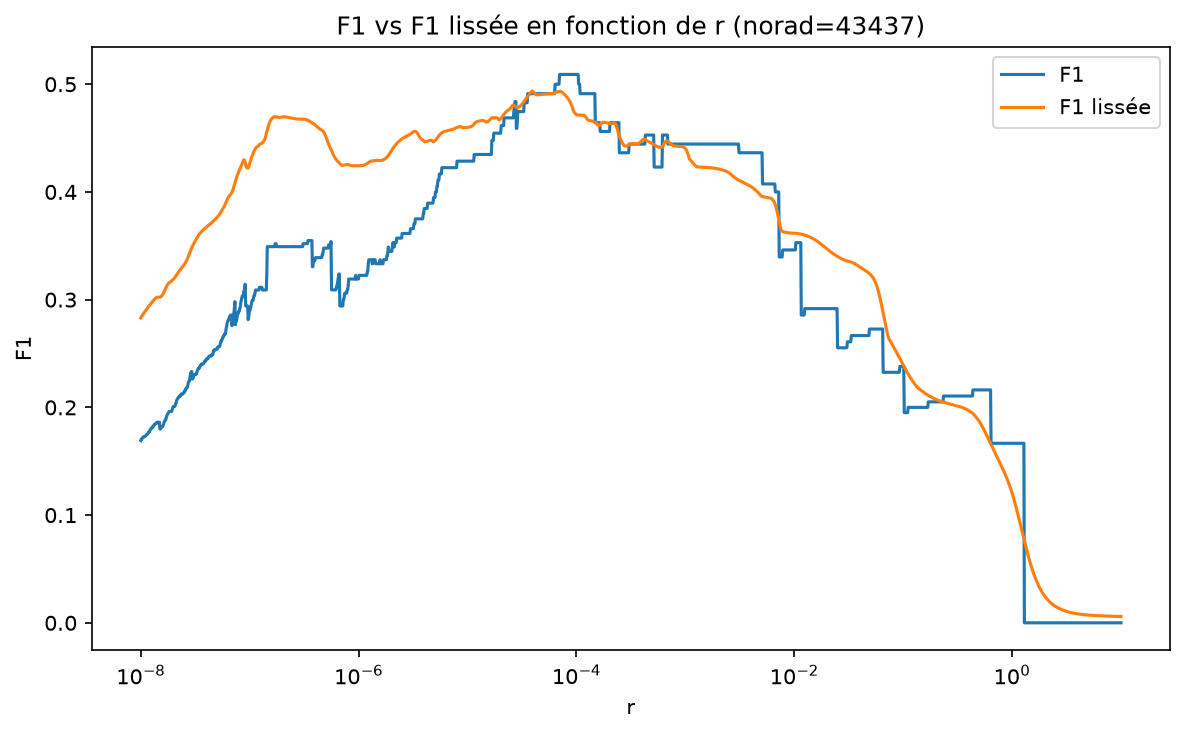
\includegraphics[width=0.85\textwidth]{figures/43437_f1_vs_r.png}
    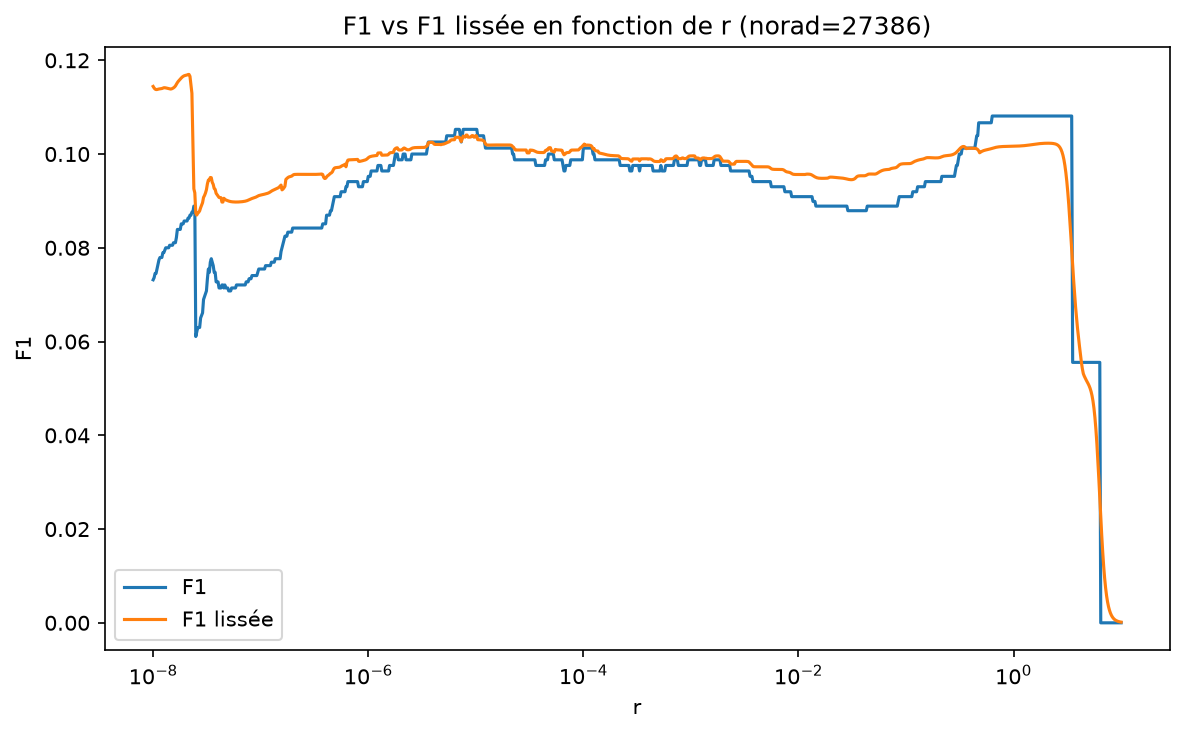
\includegraphics[width=0.85\textwidth]{figures/27386_f1_vs_r.png}
    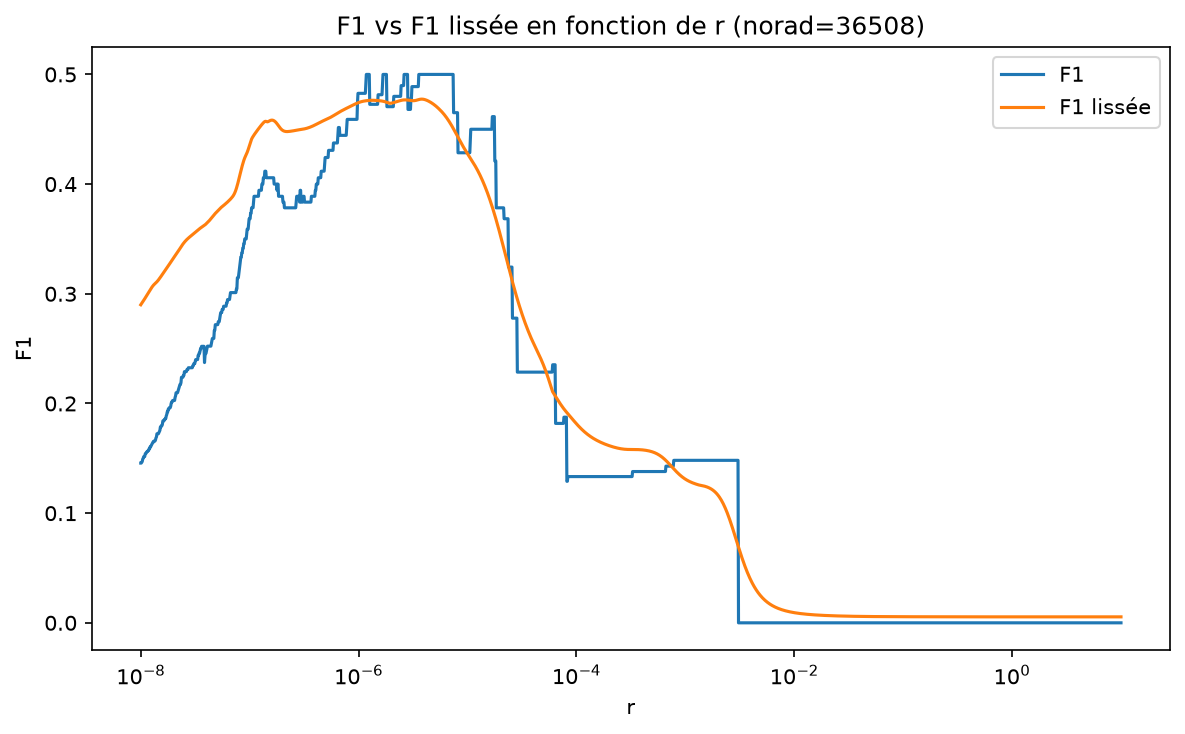
\includegraphics[width=0.85\textwidth]{figures/36508_f1_vs_r.png}
    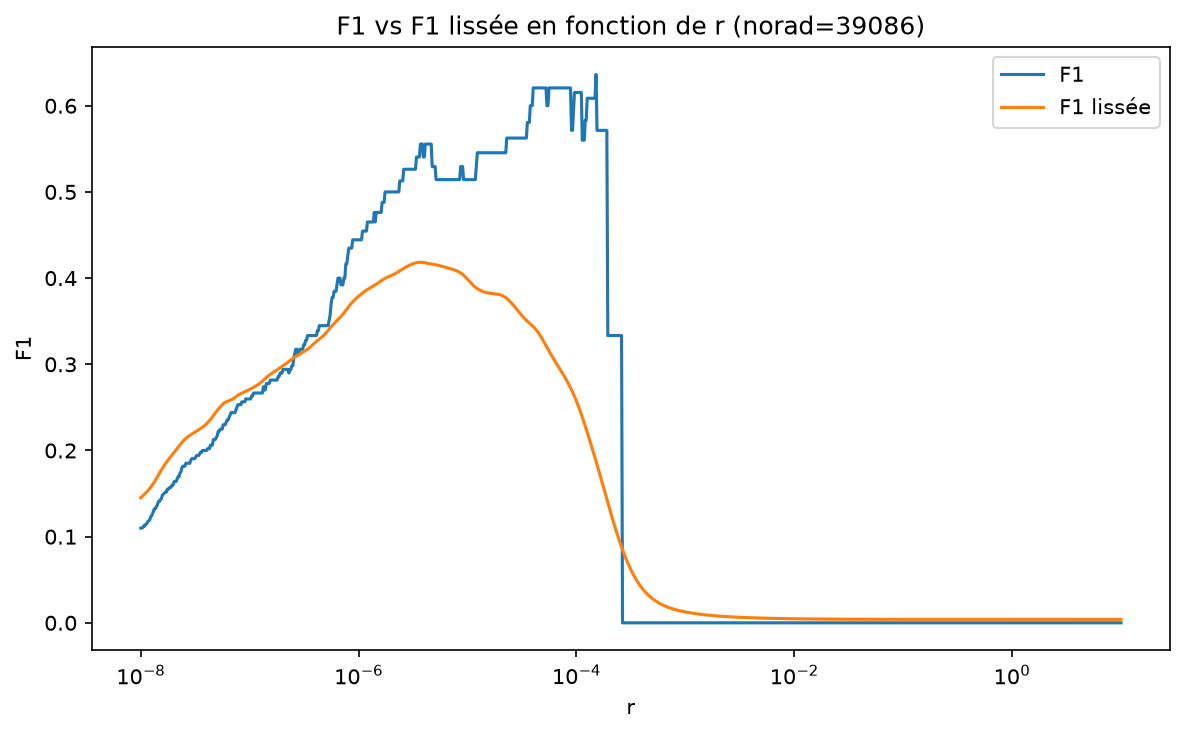
\includegraphics[width=0.85\textwidth]{figures/39086_f1_vs_r.png}
\end{center}

On cherche donc le minimum de la métrique lissée par des techniques classiques d'optimisation de fonctions régulières.

\end{document}
